%%% Local Variables:
%%% mode: latex
%%% TeX-master: t
%%% End:

%\documentclass[bachelor,nofonts]{thuthesis}
\documentclass[master]{thuthesis}
%\documentclass[doctor]{thuthesis}
% \documentclass[%
%   bachelor|master|doctor|postdoctor, % mandatory option
%   winfonts|nofonts|adobefonts, % mandatory only for bachelor and Linuxer
%   secret,
%   openany|openright,
%   arialtoc,arialtitle]{thuthesis}
% 当使用 XeLaTeX 编译时,本科生、Linux 用户需要加上 nofonts 选项;
% 当使用 PDFLaTeX 编译时,adobefonts 选项等效于 winfonts 选项(缺省选项)。

% 所有其它可能用到的包都统一放到这里了,可以根据自己的实际添加或者删除。
\usepackage{thutils}
\usepackage{lineno,hyperref}
% 你可以在这里修改配置文件中的定义,导言区可以使用中文。
% \def\myname{薛瑞尼}
\usepackage{amsmath}
\begin{document}

% 定义所有的eps文件在 figures 子目录下
\graphicspath{{figures/}}


%%% 封面部分
\frontmatter

%%% Local Variables:
%%% mode: latex
%%% TeX-master: t
%%% End:

% 中国海洋大学研究生学位论文封面
% 参考:中国海洋大学研究生学位论文书写格式20130307.doc

% 为避免出现错误,下面保留[清华大学学位论文模板原有定义无需修改],
% 请直接跳到后面[中国海洋大学学位论文模板部分请根据自己情况修改]。

%%%%%%%%%%%%%%%%%%%%%%[清华大学学位论文模板原有定义无需修改]%%%%%%%%%%%%%%%%%%%%%%%
\secretlevel{绝密} \secretyear{2100}

\ctitle{清华大学学位论文 \LaTeX\ 模板\\使用示例文档}
% 根据自己的情况选,不用这样复杂
\makeatletter
\ifthu@bachelor\relax\else
  \ifthu@doctor
    \cdegree{工学博士}
  \else
    \ifthu@master
      \cdegree{工学硕士}
    \fi
  \fi
\fi
\makeatother


\cdepartment[计算机]{计算机科学与技术系}
\cmajor{计算机科学与技术}
\cauthor{薛瑞尼} 
\csupervisor{郑纬民教授}
% 如果没有副指导老师或者联合指导老师,把下面两行相应的删除即可。
\cassosupervisor{陈文光教授}
\ccosupervisor{某某某教授}
% 日期自动生成,如果你要自己写就改这个cdate
%\cdate{\CJKdigits{\the\year}年\CJKnumber{\the\month}月}

% 博士后部分
% \cfirstdiscipline{计算机科学与技术}
% \cseconddiscipline{系统结构}
% \postdoctordate{2009年7月——2011年7月}

\etitle{An Introduction to \LaTeX{} Thesis Template of Tsinghua University} 
% 这块比较复杂,需要分情况讨论:
% 1. 学术型硕士
%    \edegree:必须为Master of Arts或Master of Science(注意大小写)
%              “哲学、文学、历史学、法学、教育学、艺术学门类,公共管理学科
%               填写Master of Arts,其它填写Master of Science”
%    \emajor:“获得一级学科授权的学科填写一级学科名称,其它填写二级学科名称”
% 2. 专业型硕士
%    \edegree:“填写专业学位英文名称全称”
%    \emajor:“工程硕士填写工程领域,其它专业学位不填写此项”
% 3. 学术型博士
%    \edegree:Doctor of Philosophy(注意大小写)
%    \emajor:“获得一级学科授权的学科填写一级学科名称,其它填写二级学科名称”
% 4. 专业型博士
%    \edegree:“填写专业学位英文名称全称”
%    \emajor:不填写此项
\edegree{Doctor of Engineering} 
\emajor{Computer Science and Technology} 
\eauthor{Xue Ruini} 
\esupervisor{Professor Zheng Weimin} 
\eassosupervisor{Chen Wenguang} 
% 这个日期也会自动生成,你要改么?
% \edate{December, 2005}

% 定义中英文摘要和关键字
\begin{cabstract}
  论文的摘要是对论文研究内容和成果的高度概括。摘要应对论文所研究的问题及其研究目
  的进行描述,对研究方法和过程进行简单介绍,对研究成果和所得结论进行概括。摘要应
  具有独立性和自明性,其内容应包含与论文全文同等量的主要信息。使读者即使不阅读全
  文,通过摘要就能了解论文的总体内容和主要成果。

  论文摘要的书写应力求精确、简明。切忌写成对论文书写内容进行提要的形式,尤其要避
  免“第 1 章……;第 2 章……;……”这种或类似的陈述方式。

  本文介绍清华大学论文模板 \thuthesis{} 的使用方法。本模板符合学校的本科、硕士、
  博士论文格式要求。

  本文的创新点主要有:
  \begin{itemize}
    \item 用例子来解释模板的使用方法;
    \item 用废话来填充无关紧要的部分;
    \item 一边学习摸索一边编写新代码。
  \end{itemize}

  关键词是为了文献标引工作、用以表示全文主要内容信息的单词或术语。关键词不超过 5
  个,每个关键词中间用分号分隔。(模板作者注:关键词分隔符不用考虑,模板会自动处
  理。英文关键词同理。)
\end{cabstract}

\ckeywords{\TeX, \LaTeX, CJK, 模板, 论文}

\begin{eabstract} 
   An abstract of a dissertation is a summary and extraction of research work
   and contributions. Included in an abstract should be description of research
   topic and research objective, brief introduction to methodology and research
   process, and summarization of conclusion and contributions of the
   research. An abstract should be characterized by independence and clarity and
   carry identical information with the dissertation. It should be such that the
   general idea and major contributions of the dissertation are conveyed without
   reading the dissertation. 

   An abstract should be concise and to the point. It is a misunderstanding to
   make an abstract an outline of the dissertation and words ``the first
   chapter'', ``the second chapter'' and the like should be avoided in the
   abstract.

   Key words are terms used in a dissertation for indexing, reflecting core
   information of the dissertation. An abstract may contain a maximum of 5 key
   words, with semi-colons used in between to separate one another.
\end{eabstract}

\ekeywords{\TeX, \LaTeX, CJK, template, thesis}
%%%%%%%%%%%%%%%%%%%%%%%%%%%%%%%%%%%%%%%%%%%%%%%%%%%%%%%%%%%%%%%%%%%%%%%%%%%%%%%%

%%%%%%%%%%%%%%%%%%[中国海洋大学学位论文模板部分请根据自己情况修改]%%%%%%%%%%%%%%%%%%%
% 中国海洋大学研究生学位论文封面
% 必须填写的内容包括(其他最好不要修改):
%   分类号、密级、UDC
%   论文中文题目、作者中文姓名
%   论文答辩时间
%   封面感谢语
%   论文英文题目
%   中文摘要、中文关键词
%   英文摘要、英文关键词
%
%%%%%[自定义]%%%%%
\newcommand{\fenleihao}{}%分类号
\newcommand{\miji}{}%密级 
                    % 绝密$\bigstar$20年 
                    % 机密$\bigstar$10年
                    % 秘密$\bigstar$5年
\newcommand{\UDC}{}%UDC
\newcommand{\oucctitle}{图像频域显著性检测}%论文中文题目
\ctitle{图像频域显著性检测}%必须修改因为页眉中用到
\cauthor{赵红苗}%可以选择修改因为仅在 pdf 文档信息中用到
\cdegree{工学硕士}%可以选择修改因为仅在 pdf 文档信息中用到
\ckeywords{\TeX, \LaTeX, CJK, 模板, 论文}%可以选择修改因为仅在 pdf 文档信息中用到
\newcommand{\ouccauthor}{赵红苗}%作者中文姓名
%\newcommand{\ouccsupervisor}{姬光荣教授}%作者导师中文姓名
%\newcommand{\ouccdegree}{博\hspace{1em}士}%作者申请学位级别
%\newcommand{\ouccmajor}{海洋信息探测与处理}%作者专业名称
%\newcommand{\ouccdateday}{\CJKdigits{\the\year}年\CJKnumber{\the\month}月\CJKnumber{\the\day}日}
%\newcommand{\ouccdate}{\CJKdigits{\the\year}年\CJKnumber{\the\month}月}
\newcommand{\oucdatedefense}{2015年05月28日}%论文答辩时间
%\newcommand{\oucdatedegree}{2009年6月}%学位授予时间
\newcommand{\oucgratitude}{谨以此论文献给我的导师和亲人!}%封面感谢语
\newcommand{\oucetitle}{Image Saliecy Detection in Frequency Domain}%论文英文题目
%\newcommand{\ouceauthor}{Haiyong Zheng}%作者英文姓名
\newcommand{\oucthesis}{\textsc{OUCThesis}}
%%%%%默认自定义命令%%%%%
% 空下划线定义
\newcommand{\oucblankunderline}[1]{\rule[-2pt]{#1}{.7pt}}
\newcommand{\oucunderline}[2]{\underline{\hskip #1 #2 \hskip#1}}

% 论文封面第一页
%%不需要改动%%
\vspace*{5cm}
{\xiaoer\heiti\oucgratitude

\begin{flushright}
---\hspace*{-2mm}---\hspace*{-2mm}---\hspace*{-2mm}---\hspace*{-2mm}---\hspace*{-2mm}---\hspace*{-2mm}---\hspace*{-2mm}---\hspace*{-2mm}---\hspace*{-2mm}---~\ouccauthor
\end{flushright}
}

\newpage

% 论文封面第二页
%%不需要改动%%
\vspace*{1cm}
\begin{center}
  {\xiaoer\heiti\oucctitle}
\end{center}
\vspace{10.7cm}
{\normalsize\songti
\begin{flushright}
{\renewcommand{\arraystretch}{1.3}
  \begin{tabular}{r@{}l}
    学位论文答辩日期:~ & \oucunderline{1.8em}{\oucdatedefense} \\
    指导教师签字:~ & \oucblankunderline{5cm} \\
    答辩委员会成员签字:~ & \oucblankunderline{5cm} \\
    ~ & \oucblankunderline{5cm} \\
    ~ & \oucblankunderline{5cm} \\
    ~ & \oucblankunderline{5cm} \\
    ~ & \oucblankunderline{5cm} \\
    ~ & \oucblankunderline{5cm} \\
    ~ & \oucblankunderline{5cm} \\
  \end{tabular}
}
\end{flushright}
}

\newpage

% 论文封面第三页
%%不需要改动%%
\vspace*{1cm}
\begin{center}
  {\xiaosan\heiti 独\hspace{1em}创\hspace{1em}声\hspace{1em}明}
\end{center}
\par{\normalsize\songti\parindent2em
本人声明所呈交的学位论文是本人在导师指导下进行的研究工作及取得的研究成果。据我所知,除了文中特别加以标注和致谢的地方外,论文中不包含其他人已经发表或撰写过的研究成果,也不包含未获得~\oucblankunderline{7cm}(注:如没有其他需要特别声明的,本栏可空)或其他教育机构的学位或证书使用过的材料。与我一同工作的同志对本研究所做的任何贡献均已在论文中作了明确的说明并表示谢意。
}
\vskip1.5cm
\begin{flushright}{\normalsize\songti
  学位论文作者签名:\hskip2cm 签字日期:\hskip1cm 年 \hskip0.7cm 月\hskip0.7cm 日}
\end{flushright}
\vskip.5cm
{\setlength{\unitlength}{0.1\textwidth}
  \begin{picture}(10, 0.1)
    \multiput(0,0)(0.2, 0){50}{\rule{0.15\unitlength}{.5pt}}
  \end{picture}}
\vskip1cm
\begin{center}
  {\xiaosan\heiti 学位论文版权使用授权书}
\end{center}
\par{\normalsize\songti\parindent2em
本学位论文作者完全了解学校有关保留、使用学位论文的规定,并同意以下事项:
\begin{enumerate}
\item 学校有权保留并向国家有关部门或机构送交论文的复印件和磁盘,允许论文被查阅和借阅。
\item 学校可以将学位论文的全部或部分内容编入有关数据库进行检索,可以采用影印、缩印或扫描等复制手段保存、汇编学位论文。同时授权清华大学“中国学术期刊(光盘版)电子杂志社”用于出版和编入CNKI《中国知识资源总库》,授权中国科学技术信息研究所将本学位论文收录到《中国学位论文全文数据库》。
\end{enumerate}
(保密的学位论文在解密后适用本授权书)
}
\vskip1.5cm
{\parindent0pt\normalsize\songti
学位论文作者签名:\hskip4.2cm\relax%
导师签字:\relax\hspace*{1.2cm}\\
签字日期:\hskip1cm 年\hskip0.7cm 月\hskip0.7cm 日\relax\hfill%
签字日期:\hskip1cm 年\hskip0.7cm 月\hskip0.7cm 日\relax\hspace*{1.2cm}}

\newpage

\pagestyle{plain}
\clearpage\pagenumbering{roman}

% 中文摘要
%%[需要填写:中文摘要、中文关键词]%%
\begin{center}
  {\sanhao[1.5]\heiti\oucctitle\\\vskip7pt 摘\hspace{1em}要}
\end{center}
{\normalsize\songti

  \indent
显著性检测在计算机视觉应用中十分广泛,如图像分割、目标识别、图像重定向及视频压缩等。频域显著性检测(谱显著性检测)具有简单、快速、高效、不依赖于分类或其他先验知识的特点,吸引了越来越多的人对它进行研究。本文详细介绍了频域算法的具体流程,对国内外提出的算法和模型进行了具体的归纳和整理。通过分析发现许多计算方法还存在着显著区域检测不均匀、显著性细节检测不理想等问题。针对这些缺点,我们提出了一种新的显著性检测算法---基于幅度谱分析的自适应显著目标检测。

我们假设自然图像是由显著区域和一些所谓的规则的区域组成,这些规则的区域被看作重复模式(非显著性)图像在空间域中周期出现的模式,证明是对应于频域幅度谱中一个或多个相应位置的尖峰。我们算法的思想是在正确尺度上利用幅度谱滤波平滑重复模式的尖峰,达到抑制图像非显著性区域,突出显著区域的目的。本文的贡献主要有:
  \begin{itemize}
    \item 通过实验分析我们发现显著区域的尺寸与最优幅度谱滤波尺度之间存在特定的关系,这对于频域显著目标检测研究具有十分重要的意义;
    \item 在尺度空间的基础上,提出了自适应最优尺度选择新的方法;
    \item 引入了一种自适应权重融合新策略,融合不同显著目标所对应的显著图,从而保留有意义的显著性信息;
    \item 本文提出的算法在与其他频域显著性检测模型进行对比时,选择的数据集更具有挑战性。
  \end{itemize}

我们在四个国际公开数据集上进行了定性定量的对比实验,证明了我们的算法较其他的谱显著性模型在有效性和优越性方面表现的更好。
}
\vskip12bp
{\xiaosi\heiti\noindent
关键词:\hskip1em 谱显著性, 显著目标检测, 幅度谱分析, 尺度空间分析}

\newpage

% 英文摘要
%%[需要填写:英文摘要、英文关键词]%%
\begin{center}
  {\sanhao[1.5]\heiti\oucetitle\\\vskip7pt Abstract}
\end{center}
{\normalsize\songti

Saliency detection is widely useful for many computer vision applications, such as image segmentation, object recognition, image retargeting, video compression, etc. Being simple, fast, effective, and independent of categories, or other forms of prior knowledge, saliency detection in the frequency domain (spectral saliency) attracts more study. This paper introduces the concrete procedure of the algorithm in frequency domain and overviews the domestic and overseas models. The analysis indicates that many computational methods can not highlight the objects uniformly or have poor contrast saliency maps. To address these issues, a novel saliency detection model---salient object detection via automatic adaptive amplitude spectrum analysis is proposed in this paper. 

The proposed model assumes that a natural image consists of several salient and many so--called regular regions which are regarded as repeated patterns (nonsaliency). The spikes in the amplitude spectrum turn out to correspond to repeated patterns in spatial domain. The idea of the proposed method is smoothing the spikes in the amplitude spectrum at an appropriate scale to suppress nonsalient patterns for saliency pop-out. The main contributions of this paper are shown as follows:
\begin{enumerate}
\item  This paper observes that the optimal scale for smoothing the amplitude spectrum shares specific relation with the size of salient region, which is very important for the research of salient region detection in frequency domain.
\item Automatic optimal scales selection based on the Spectrum Scale--Space is proposed in this paper.
\item  A new strategy of adaptive weighted combination to incorporate meaningful saliency maps, produced by different optimal scales for multiple salient objects adaptively, is introduced for retaining meaningful saiency information.
\item The selected datasets are more challenging when compared the proposed methods with selected state-of-art saliency models.
\end{enumerate}

The performance evaluation of quantitative and qualitative comparisons on four challenging popular benchmark data sets validates that the proposed method outperforms the existing spectral saliency models in terms of effectiveness and superiority.
}
\vskip12bp
{\xiaosi\heiti\noindent 
\textbf{Keywords:\enskip spectral saliency, salient object detection, amplitude spectrum analysis, scale sapce analysis}}
%%%%%%%%%%%%%%%%%%%%%%%%%%%%%%%%%%%%%%%%%%%%%%%%%%%%%%%%%%%%%%%%%%%%%%%%%%%%%%%%

% 设置 PDF 文档的作者、主题等属性
\makeatletter
\thu@setup@pdfinfo
\makeatother
%\makecover

% 目录
\tableofcontents

% 符号对照表
%\input{data/denotation}


%%% 正文部分
\mainmatter

%%% Local Variables:
%%% mode: latex
%%% TeX-master: t
%%% End:

\chapter{绪论}
\label{cha1}

\section{研究背景及意义}
\label{1_1}

人类及其他灵长类动物在面对复杂场景时能够简单快速的找到自己感兴趣或比较显著的区域,并对其进行优先处理,这个过程叫做视觉注意。视觉注意机制是视觉系统本身的一种属性,是为适应环境而进化的产物,在视觉信息处理过程中有着十分重要的意义。每天人类及其他灵长类动物的眼睛都要接受海量的信息,但是视觉信息处理能力是有限的,视觉系统无法将图像中所有的信息都进行处理,并且我们所关注的内容只占一小部分。所以,通过视觉注意这种机制,我们可以对感兴趣的信息进行选择性处理,并且给予不同的处理级别,从而减小了信息处理的复杂性,节省了时间,在很大程度上提高了视觉系统的信息处理效率。

视觉注意根据心理和生理机制可以分为两种,一种是自底向上的视觉注意,另一种是自顶向下的视觉注意。自底向上的视觉注意不受意识控制,独立于具体任务,靠数据进行驱动,处理信息时速度相对比较快,比如你的面前有一堆绿色的苹果,其中只有一个苹果是红色的,当这些苹果映入你眼帘时,你会不由自主的只注视那只红色的苹果。自顶向下的视觉注意取决大脑高级皮层先验信息的反馈,因此受意识支配,处理信息的速度相对较慢,比如还是前面的例子,这一堆绿苹果中只有一个红苹果,但是也包含一个烂了的苹果,现在你准备把这个烂苹果从苹果堆里挑出来,因此当你面对这一堆苹果的时候,你就会将注意力集中在坏掉的苹果上,而不是红色或绿色的苹果。

视觉注意机制是一个多学科多交叉的领域,自研究以来得到了许多学科研究者的关注,如:神经科学、生理学、心理学以及计算机科学等。其中,将视觉注意引入到计算机领域称为显著性检测,即检测出图像的显著性信息,忽略冗余信息,使图像处理的结果更加符合人类的视觉感受。随着计算机科学技术的发展,视觉注意计算模型逐渐成为计算机视觉及图像处理研究者感兴趣的热点,并越来越多的应用到计算机视觉领域,如图像分割、目标识别、图像重定向及视频压缩等。

空间域视觉注意仿生模型较好的模拟了人类的视觉注意机制,但是由于过多地模拟这种生理机制使得计算量相对较大,比较耗时。基于信息论和统计等显著性检测模型需要估测概率密度或建立概率模型,引入大量参数,并且计算效率比较低,因此,不适于工程性应用。频域处理具有简单、高效及参数设置少的特点,可以对图像进行实时性处理,所以自底向上的频域视觉注意模型对于显著性检测是很好的选择。

\section{国内外研究现状}
\label{1_2}

视觉注意在计算机领域的研究被称为显著性检测。目前,有关显著性检测的研究可以大致分为两类:注视焦点预测和显著性目标检测\cite{ChengMingMingCVPR2014BING,LiYinCVPR2014Secrets}。注视焦点预测旨在通过计算显著图来模拟人眼观测点。在Koch与Ullman\cite{Koch1987Shifts}提出的特征融合理论和神经生物学框架的启发下,Itti等人\cite{IttiTPAMI1998Model}建立了第一个自底向上的显著性检测计算模型。该模型利用线性滤波的方法提取图像的颜色、亮度和方向等特征得到多尺度的特征图高斯金字塔,通过中央周围差和归一化算子获得特征显著图,然后将这些特征显著图通过线性融合机制融合成显著图,采用赢者全取的策略支配视觉焦点的转移。该模型较为完整的模拟了视觉注意机制,在计算机显著性检测领域具有里程碑的作用。注视焦点模型获得了很大的改进和发展\cite{JuddMIT2012Benchmark,BorjiTIP2013Quantitative,BorjiICCV2013Analysis,BorjiTPAMI2013State,VigCVPR2014Large},但是预测的结果往往趋向于突显边缘和角点等纹理较密集的区域,而非整个目标,因此,该种模型应用性不高\cite{ChengMingMingCVPR2014BING}。

显著目标检测是用来检测给定场景中最显著、最能引起人注意的整个物体,并将它完整的分割出来\cite{BorjiECCV2012Salient,LiYinCVPR2014Secrets}。Liu等人\cite{LiuTieCVPR2007Learning}通过条件随机场将局部、区域和全局的显著目标特征融合起来。Achanta等人\cite{AchantaCVPR2009Frequency}通过调频的方法,利用颜色和亮度信息进行显著区域检测。Cheng等人\cite{ChengMingMingCVPR2011Global}提出了基于区域对比度的显著性检测方法。最近,更多的研究方法\cite{BorjiECCV2012Salient}关注于如何使得显著性检测结果更精确、更鲁棒,如基于滤波器方程的方法\cite{PerazziCVPR2012filters}、判别区域特征融合的方法\cite{JiangHuaizuCVPR2013Discriminative}、基于图的流型排序\cite{YangChuanCVPR2013Manifold}、分层的方法\cite{YanQiongCVPR2013Hierarchical}和子模框架\cite{JiangZhuolinCVPR2013Submodular},另外还有统计纹理特征的方法\cite{ScharfenbergerCVPR2013Statistical}、有效数据表达\cite{ChengMingMingICCV2013Efficient}、基于上下文超图建模\cite{LiXiICCV2013Contextual}、布尔图的方法\cite{ZhangJianmingICCV2013Boolean}、基于马尔可夫链的方法\cite{JiangBowenICCV2013Markov}、稀疏性表达的方法\cite{LiXiaohuiICCV2013Dense}、偏微分方程学习的方法\cite{LiuRishengCVPR2014Adaptive}以及光场的方法\cite{LiNianyiCVPR2014Light}等等。显著目标检测强调检测出整个显著物体,因此它在计算机视觉领域具有广泛的应用\cite{BorjiTPAMI2013State},比如图像场景分析、内容感知、图像编辑、图像视频压缩等。尽管显著目标检测的精度越来越高,但在处理的过程中特征选择越来越多、算法越来越复杂,使得计算量越来越大,造成计算效率越来越低,因此,不便于进行实时性处理。

为了更为简单、快速、有效并且不依赖于分类或其他先验知识,频域显著性检测吸引了越来越多人的研究。Hou和Zhang首先将显著性检测引入到频域中,提出了谱剩余的显著性检测算法(SR)\cite{HouXiaodiCVPR2007Residual}。经过分析,Guo等人\cite{GuoChenleiCVPR2008Spatio}认为去掉幅度谱,只保留相位谱就可以恢复出图像的显著图而无需利用剩余谱,得出的结果跟SR算法的几乎一样。他们还将傅里叶变换扩展为四元数傅里叶变换,考虑到了图像的颜色、亮度等信息,将它们结合在一个变换中,提出了相位谱四元数傅里叶变换(PQFT)。之后,频域显著性模型又得到了更多的扩展,如脉冲主成分分析的脉冲离散余弦变换模型(PCA)\cite{YuICDL2009Spatio}和频域分解归一化模型(PDN)\cite{BianCognNeurodyn2010Visual}。以上方法虽然取得了一定的效果,但是他们仅仅可以检测出边缘、纹理复杂的较小区域,对于目标较大的区域检测效果并不理想。直到2013年,Li等人提出了基于谱尺度空间的显著性检测算法(HFT)\cite{LiJianTPAMI2013Scale}解决了这个问题,该算法将背景看作重复模式,对应于频域幅度谱的尖刺,通过不同尺度的高斯滤波器对幅度谱进行平滑,达到抑制背景、突出前景显著目标的目的。

\section{本文主要工作及安排}
\label{1_3}

本文主要对自底向上的频域显著性检测算法进行了研究,总结了国际上现有的频域显著性检测处理方法,并提出了基于自适应幅度谱分析的谱显著性检测算法。本文的主要安排如下:

第一章为绪论部分,主要对频域显著性检测算法的背景、意义及国内外研究现状进行介绍,并对全文的主要工作及安排进行了说明。

第二章介绍基于频域处理的显著性检测。详细介绍了算法的设计框架和流程,包括图像预处理、时频变换、谱处理、图像后续处理等,对每一个环节进行详细的分析和归纳。

第三章将国内外频域显著性检测方法进行整理和总结,完成对频域显著性检测经典算法的综述。

第四章针对频域显著区域检测问题设计了算法,详细介绍了算法的设计框架,并结合实际处理结果说明了方法的有效性,并通过在大量图像数据集上的实验证明了算法的优越性。

第五章对全文的工作进行了总结,并指出工作中存在的问题对以后的工作提出了展望。

\section{本章小结}
\label{1_4}

本章主要介绍了频域显著性检测的背景和意义,同时分析了国内外研究的现状,并对全文的工作和安排进行了介绍。



%%% Local Variables: 
%%% mode: latex
%%% TeX-master: t
%%% End: 

\chapter{频域显著性检测}
\label{cha2}

随着计算机技术的进步和发展,图像显著性检测的要求越来越高。频域显著性检测技术较空间域的处理更适应于降低计算的复杂度,提高计算的准确度和效率,避免过多的资源浪费。图像由空间域转换到频域进行处理必须选择适当的时频转换,如傅里叶变换、小波变换等。不管图像是怎样的,图像的空间域信息在转换到频域时都被保留在幅度谱和相位谱中,当它们之间进行相互转换时信息不会发生丢失。频域显著性检测一般是将输入的图像进行预处理,如将图像转换到不同颜色空间来提取各种特征、图像尺度变换等; 然后进行时频转换把图像转换到频域,得到图像相应的谱成分; 再对相应的谱进行一定的处理得到处理后的谱; 然后将处理后的谱结合在一起通过反变换将图像由频域转换到空间域;最后,经过图像的后处理得到最终的显著图。频域显著性检测的一般步骤见图~\ref{图2_1}。接下来的内容将针对频域显著性检测的各个阶段进行归纳和综述。

\begin{figure}[h]
  \centering
  \includegraphics[height=0.6cm]{图2_1}
  \caption{频域显著性检测的一般步骤}
  \label{图2_1}    
\end{figure}

%============================================================================================================
\section{预处理}
\label{2_1}

大多数频域显著性检测模型在进行处理时,首先要进行图像的预处理,包括特定颜色空间转换用来提取特征、尺度变换等。下面将对图像的彩色空间和尺度变换进行整理和总结。

%-------------------------------------------------------------------------------------------------------------
\subsection{RGB彩色模型}
\label{2_1_1}

RGB彩色空间是目前运用最广泛的颜色模型之一,是工业界一种颜色标准,被大多数人所熟识。它是通过对红、绿、蓝三原色亮度的变化及他们相互之间的叠加得到各种各样颜色的,该标准几乎包含了人类视觉所能感知的所有颜色。

\begin{figure}[t]
  \centering
  \includegraphics[height=5cm]{图2_2}
  \caption{RGB彩色模型}
  \label{图2_2}    
\end{figure}

图~\ref{图2_2}所示的即为RGB彩色模型对应的坐标系~\cite{ZhangZheng2010book}。在立方体的3个顶点上分别是红、绿、蓝,青、黄和深红分别位于另外的3个角的顶点上,黑色位于坐标原点,白色则在离原点最远的顶点上,灰度级沿着这两点的连线依次分布,不同的颜色位于立方体的内部和边缘上,因此所有的颜色都可以通过一个3维向量进行表示。例如,假设将所有颜色归一化为$[0,1]$,红色可以表示为$(1,0,0)$,白色可以表示为$(1,1,1)$。

在Matlab实验中,可以直接将图像的R、G、B颜色特征提取出来,如图~\ref{图2_3},RGB彩色空间常用于图像/视频采集、图像表达和图像显示等。

\begin{figure}[b]
\begin{minipage}{0.24\textwidth}
  \centering
  \includegraphics[height=2cm]{图2_3_a}
  \label{图2_3_a}
\end{minipage}\hfill
\begin{minipage}{0.24\textwidth}
  \centering
  \includegraphics[height=2cm]{图2_3_b}
  \label{图2_3_b}
\end{minipage}
\begin{minipage}{0.24\textwidth}
  \centering
  \includegraphics[height=2cm]{图2_3_c}
  \label{图2_3_c}
\end{minipage}
\begin{minipage}{0.24\textwidth}
  \centering
  \includegraphics[height=2cm]{图2_3_d}
  \label{图2_3_d}
\end{minipage}
  \caption{图像的RGB颜色模型例子。从左至右分别为原图像、R通道图像、G通道图像和B通道图像。}
  \label{图2_3} 
\end{figure}

%-------------------------------------------------------------------------------------------------------------
\subsection{Lab彩色模型}
\label{2_1_2}

Lab彩色模型是经由国际照明委员会(CIE)制定的一种颜色模式,自然界存在的任何色彩都可在Lab空间中表达出来~\cite{ZhangZheng2010book}。Lab被设计来接近人类视觉,该空间中的数值表示正常视力的人可以看到的所有颜色。Lab描述的并不是生成颜色所需要的特定色料的数量,而是颜色的显示方式,因此,它被看作与设备无关的颜色模型。

Lab模型是有关亮度L和有关彩色a和b三个部分组成。L代表亮度,a代表从红色/品红色到绿色的部分,b代表从黄色到蓝色的部分。L的值从$0$至$100$,分别由纯黑转为纯白,a和b的取值范围都是$[127,-128]$,计算表达式如下:
\begin{linenomath}
\begin{align}
L^{*} &= 116f\big(\frac{Y}{y_{n}}-16\big)\label{式2_1}\\
a^{*} &= 500\big[f(\frac{X}{X_{n}})-f(\frac{Y}{Y_{n}})\big]\label{式2_2}\\
b^{*} &= 200\big[f(\frac{Y}{Y_{n}})-f(\frac{Z}{Z_{n}})\big]\label{式2_3}\\
y &= \left\{ \begin{array}{ll}
t^{\frac{1}{3}}, & \textrm{if $t>(\frac{6}{29})^{3}$}\\
\frac{1}{3}(\frac{29}{6})^{2}t+\frac{4}{29}, & \textrm{if $t\leq (\frac{6}{29})^{3}$}
\end{array} \right.\label{式2_4}\\
f(t) &= \left\{ \begin{array}{ll}
t^{\frac{1}{3}}, & \textrm{if $t>(\frac{6}{29})^{3}$}\\
\frac{1}{3}(\frac{29}{6})^{2}t+\frac{4}{29}, & \textrm{if $t\leq (\frac{6}{29})^{3}$}
\end{array} \right.\label{式2_5}
\end{align}
\end{linenomath}
其中,$X_{n}$,$Y_{n}$和$Z_{n}$分别是CIE XYZ彩色空间的三个值,图~\ref{图2_4}即为Lab彩色空间图,Lab彩色空间常用于颜色光适应、图像压缩和色彩差度量等。
\begin{figure}[h]
  \centering
  \includegraphics[height=5cm]{图2_4}
  \caption{Lab彩色空间图}
  \label{图2_4}    
\end{figure}

%-------------------------------------------------------------------------------------------------------------
\subsection{IRGBY彩色模型}
\label{2_1_3}

在人类视觉系统中,颜色主要有颜色拮抗系统进行表示,即神经细胞对颜色的处理具有双接抗的性质,一种颜色可以使细胞产生兴奋,它所对应的拮抗颜色可以抑制该细胞的兴奋~\cite{Engel1997Colour}。经过研究发现,视皮层中有四种彩色拮抗对,分别是红绿、绿红、蓝黄和黄蓝,因此,IRGBY彩色模型在图像处理中的应用也非常多,如显著性检测、图像/视频压缩等。IRGBY颜色空间定义如下:假设$r$,$g$和$b$分别代表红、绿、蓝三种原色,四种颜色特征分别定义为:
\begin{linenomath}
\begin{align}
\textrm{Red:$R=r-\frac{g+b}{2}$,}\label{式2_6}\\
\textrm{Green:$G=g-\frac{r+b}{2}$,}\label{式2_7}\\
\textrm{Blue:$B=b-\frac{r+g}{2}$,}\label{式2_8}\\
\textrm{Yellow:$Y=\frac{r+g}{2}-\frac{|r+g|}{2}-b$.}\label{式2_9}
\end{align}
\end{linenomath}
亮度通道$I$是红、绿、蓝三原色的平均,在显著性检测中,只需对拮抗颜色取绝对值就可以表示出两种拮抗颜色中相对兴奋的那一种。因此,红绿和绿红可以用一个公式表示,蓝黄和黄蓝可以用一个公式表示:
\begin{linenomath}
\begin{align}
RG &= \big|R-G\big|\label{式2_10}\\
BY &= \big|B-Y\big|\label{式2_11}\\
I &= \frac{r+g+b}{3}\label{式2_12}
\end{align}
\end{linenomath}

%-------------------------------------------------------------------------------------------------------------
\subsection{图像尺度调整模型}
\label{2_1_4}

在显著性检测处理初期,许多模型都会首先将图像进行多尺度调整。例如,原图像为$500×500$像素的图像,经过调整后变为$64×64$大小的图片,这样做的目的~\cite{ZhangLiming2010Book}包括两个方面:一是为了加快图像的处理速度,自底向上的显著性检测只是将图像显著部分突出出来,并不会太注重图像的细节,因此不会对图像处理效果产生必要的影响; 另外,调整图像分辨率可以将图像高频区域的噪声抑制掉,从而更有利于显著性的检测。图像内插法是最基本的调整图像大小的方法。

图像内插广泛应用于放大、收缩、旋转和几何校正等任务中,是基本的图像重取样方法。从根本上来看,图像内插是用已知数据来估计未知位置的数值处理~\cite{Gonzalez2005book}。

最近邻内插法是最简单的一种插值方法,它是把原图像中最近邻的灰度赋给每个新位置,也就是让变换后像素的灰度值等于离它最近的输入像素的灰度值。举一个简单的例子,假设大小为$300\times 300$的图像需要放大$2$倍到$600\times 600$像素,则可以假想创建一个$600\times 600$的网格,且网格之间具有大小相同的间隔,然后将其进行收缩,让它可以准确的和原图像匹配起来。很明显,收缩后的$600\times 600$网格的像素之间的间隔小于原图像的间隔,为了对覆盖后的每一点赋予灰度值,需要在原图像中找到最近的像素,然后把该像素的值赋给$600\times 600$中的新像素,完成对网格中所有点赋值后,就把图像扩展到之前规定的大小,从而得到尺度调整后的图像。最近邻内插法虽然简单,但它可能会产生失真缺陷,在实际应用中不常用。

双线性内插法~\cite{WangShen2008double}是用四个最近邻估计给定位置的灰度。令$(x,y)$是要赋予灰度值的位置,也就是前面最近邻内插法描述的网格点的坐标,然后令$v(x,y)$代表灰度值。对于双线性内插法,所赋的值是由公式$v(x,y)=ax+by+cxy+d$得到,其中四个系数的值是由四个用$(x,y)$点的最近邻点写出的未知方程来确定~\cite{Gonzalez2005book}。双线性内插法要比最近邻法得到的效果好很多,结果基本会让人满意,但计算量会增加。

双三次内插法是复杂度较高的方法它包括十六个最近邻点,赋给点$(x,y)$的灰度值是利用下式得到的:
\begin{equation}
v(x,y)=\sum_{i=0}^{3}\sum_{j=0}^{3}a_{ij}x^{i}y^{i}
\label{式2_13}
\end{equation}
其中,$16$个系数可由$16$个用$(x,y)$点的最近邻点写出的未知方程来确定。双三次内插法在保持图像细节方面要比双线性内插法的效果较好,许多商业图像内插标准程序都用的双三次内插方法,如Adobe Photoshop和Corel Photopaint等。
%标准图像$I$尺度转换表达式为:
%\begin{equation}
%I'=\textrm{resize$(I)$}
%\label{式2_13}
%\end{equation}

%\subsection{各种频域显著性检测模型前期处理方法}
%\label{subsec:fifth}
%-------------------------------------------------------------------------------------------------------------
%\subsection{本章小节}
%\label{sec:fifth}

%本章详细介绍了频域显著性检测算法前期处理的各种方法。这些方法包括彩色模型的建立用来提取图像的相关特征,图像分辨率尺度变换用来加快图像处理速度以及抑制图像噪声。其中,彩色模型的建立包括RGB彩色模型、Lab彩色模型和IRGBY彩色模型。本章对这些方法的原理和步骤进行了介绍。

%=============================================================================================================
\section{时频变换}
\label{2_2}

频域显著性检测主要是利用图像的空间域信息在频域进行处理。在大多数情况下,空间域处理和频域处理可以看作对图像显著性检测问题殊途同归的两种解决方式。而在另一些情况下,有些显著性检测问题更适合在频域中完成。频域显著性检测的优势在于:一方面可以加快图像显著性检测的速度、提高检测效率,有利于图像进行实时性处理; 另一方面,频域处理为显著性检测提供了新的思路,通过分析图像显著性区域在频域幅度谱和相位谱的分布特点,获得显著性检测的新方法。要进行频域处理,就需要对图像进行时频的相互转换。图像的时频变换包括傅里叶变换,离散余弦变换以及他们的扩展,包括四元数傅里叶变换和四元数离散余弦变换,小波变换等,下面将分别介绍图像时频变换。

%-------------------------------------------------------------------------------------------------------------
\subsection{傅里叶变换}
\label{2_2_1}

法国数学家傅里叶发现任何周期函数只要满足一定的条件(狄利赫里条件)都可以用正弦和余弦函数的加权和来表示~\cite{ZhangZheng2010book}。傅立叶变换提供了一种变换到频率域的手段,用傅里叶变换表示的函数特征可以完全利用傅里叶反变换进行重建,不容易丢失信息。

一维函数$f(x)$(其中$-\propto<x<\propto$)的傅里叶变换为:
\begin{linenomath}
\begin{align}
F(u)=\int^{\propto}_{-\propto}f(x)e^{-i2\pi ux}dx
\label{式2_14}
\end{align}
\end{linenomath}
根据$F(u)$可以通过傅里叶反变换的到$f(x)$:
\begin{linenomath}
\begin{align}
f(x)=\int^{\propto}_{-\propto}F(u)e^{i2\pi ux}du
\label{式2_15}
\end{align}
\end{linenomath}
上述两个式子就是通常提到的傅里叶变换对。对于一维函数$f(x)$(其中$x=0,1,2,\dots,M-1$)的傅里叶变换的离散形式为:
\begin{linenomath}
\begin{align}
F(u)=\sum^{M-1}_{x=0}f(x)e^{-i2\pi ux/M}, u=0,1,2,\dots,M-1
\label{式2_16}
\end{align}
\end{linenomath}
相应的反变换为:
\begin{linenomath}
\begin{align}
f(x)=\frac{1}{M}\sum^{M-1}_{x=0}F(u)e^{i2\pi ux/M},u=0,1,2,\dots,M-1
\label{式2_17}
\end{align}
\end{linenomath}
有了一维的基础,连续傅里叶变换及其反变换推广到二维分别为:
\begin{linenomath}
\begin{align}
F(u,v) &= \int^{\propto}_{-\propto}\int^{\propto}_{-\propto}f(x,y)e^{-i2\pi (ux+vy)}dxdy\label{式2_18}\\
f(x,y) &= \int^{\propto}_{-\propto}\int^{\propto}_{-\propto}F(u,v)e^{i2\pi (ux+vy)}dudv\label{式2_19}
\end{align}
\end{linenomath}
而在数字图像处理中,往往研究的是二维离散函数的傅里叶变换,则二维离散傅里叶变换及反变换公式为:
\begin{linenomath}
\begin{align}
F(u,v) &= \sum^{M-1}_{x=0}\sum^{N-1}_{y=0}f(x,y)e^{-j2\pi (ux+vy)}dxdy\label{式2_20}\\
f(x,y) &= \sum^{M-1}_{u=0}\sum^{N-1}_{v=0}F(u,v)e^{j2\pi (ux+vy)}dudv\label{式2_21}
\end{align}
\end{linenomath}
相对于空间域的变量$x$、$y$,这里的$u$、$v$则是变换域或者说是频率域的变量。傅里叶变换的极坐标的表示形式为:
\begin{equation}
F(u,v)=\Vert F(u,v)\Vert e^{j\phi(u,v)}
\label{式2_22}
\end{equation}
其中,$\Vert F(u,v)\Vert$代表图像的幅度谱,$\phi(u,v)$代表图像的相位谱。图像的频率表征了图像中灰度变化的剧烈程度,图~\ref{图2_5}展示了图像傅里叶变换的效果图。
\begin{figure}[t]
  \centering%
  \begin{subfigure}{3cm}
    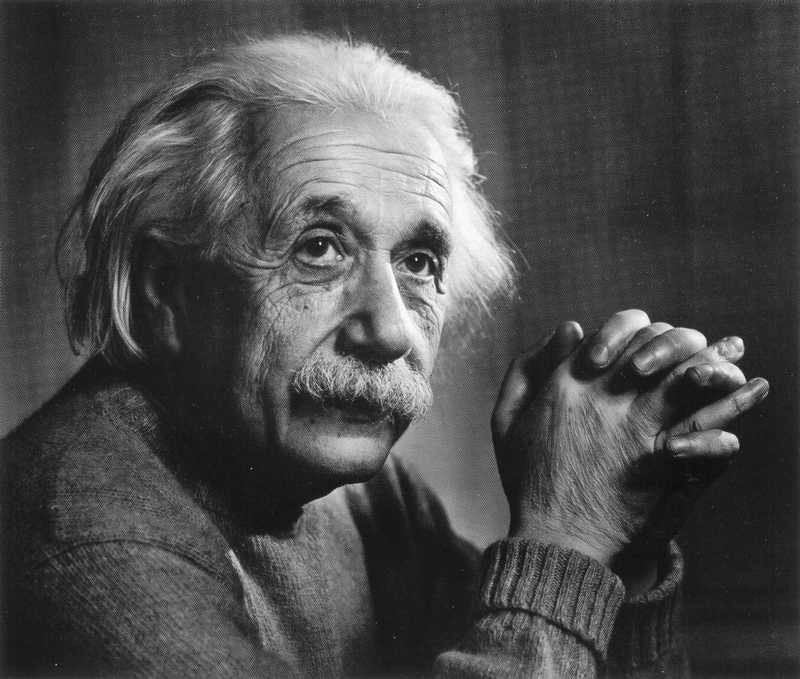
\includegraphics[height=3cm]{图2_5图2_6_a}
%    \caption{原图像}
  \end{subfigure}
  \hspace{4em}%
  \begin{subfigure}{0.25\textwidth}
    \includegraphics[height=3cm]{图2_5_b}
%    \caption{图像的离散余弦变换}
  \end{subfigure}
  \caption{图像的傅里叶变换图例。左边是原始图像,右边是对应的傅里叶谱。}
  \label{图2_5} 
\end{figure}

二维傅里叶变换图像信号能量将集中在矩阵的四个角上,例子中的频谱是经过平移之后的图像,平移之后中间部分是低频,低频亮度越大说明能量越大,对于图像而言,能量大多数集中在低频区域,而且能量越低越稳定~\cite{Gonzalez2005book}。值得说明的是,在显著性检测算法中,尤其计算尺寸较大的图像,为了提高计算效率,因此会选择傅里叶变换的快速形式,即快速傅里叶变换(FFT)用来获得图像的离散频域谱。有关图像频域幅度谱和相位谱我们将在第~\ref{2_3}节进行具体的分析和介绍。

%-------------------------------------------------------------------------------------------------------------
\subsection{离散余弦变换}
\label{2_2_2}

根据上一节我们知道,离散傅里叶变换是一种复数运算,离散实偶函数的傅里叶变换只含实的余弦项,于是构造了一种实数域的变换--离散余弦变换(DCT)~\cite{Rao2014book}。离散余弦变换的长度大概是离散傅里叶变换长度的一半,除了具有一般的正交变换性质外,其变换阵的基向量比较接近于Toeplitz矩阵的特征向量,大部分自然信号的能量大都集中在离散余弦变换之后的低频部分,DCT是语音信号、图像信号变换最佳正交变换。目前,在一系列视频压缩编码的国际标准建议中是一个基本的处理模块。

对于一幅图像$M×N$,二维离散余弦变换的表示形式为:
\begin{linenomath}
\begin{align}
F(0,0) &= \frac{1}{\sqrt{MN}}\sum_{x=0}^{M-1}\sum_{y=0}^{N-1}f(x,y)\label{式2_23}\\
F(0,v) &= \frac{\sqrt{2}}{\sqrt{MN}}\sum_{x=0}^{M-1}\sum_{y=0}^{N-1}f(x,y)cos\frac{(2y+1)v\pi}{2N}\label{式2_24}\\
F(u,0) &= \frac{\sqrt{2}}{\sqrt{MN}}\sum_{x=0}^{M-1}\sum_{y=0}^{N-1}f(x,y)cos\frac{(2x+1)u\pi}{2N}\label{式2_25}\\
F(u,v) &= \frac{2}{\sqrt{MN}}\sum_{x=0}^{M-1}\sum_{y=0}^{N-1}f(x,y)cos\frac{(2x+1)u\pi}{2N}cos\frac{(2y+1)v\pi}{2N}\label{式2_26}
\end{align}
\end{linenomath}
二维离散余弦反变换形式为:
\begin{linenomath}
\begin{align}
\lefteqn{ f(x,y)=\frac{1}{\sqrt{MN}}F(0,0)+\frac{\sqrt{2}}{\sqrt{MN}}\sum_{v=1}^{N-1}F(0,v)cos\frac{(2y+1)v\pi}{2N}+\frac{\sqrt{2}}{\sqrt{MN}}\sum_{u=1}^{M-1}F(u,0){} }\nonumber\\
& & {}cos\frac{(2x+1)v\pi}{2N}+\frac{2}{\sqrt{MN}}F(u,v)cos\frac{(2x+1)v\pi}{2N}cos\frac{(2y+1)v\pi}{2N}
\label{式2_27}
\end{align}
\end{linenomath}

\begin{figure}[t]
  \centering%
  \begin{subfigure}{3cm}
    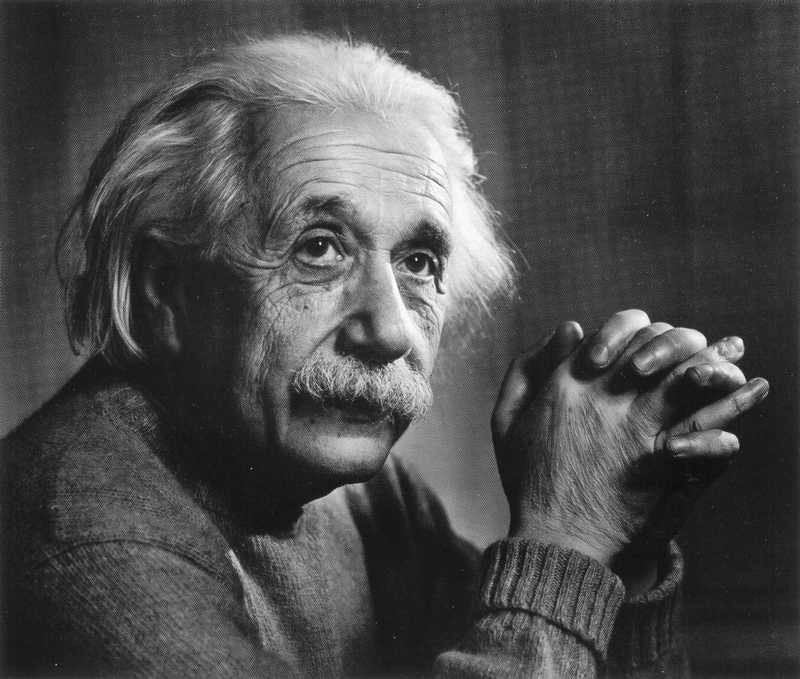
\includegraphics[height=3cm]{图2_5图2_6_a}
%    \caption{原图像}
  \end{subfigure}
  \hspace{4em}%
  \begin{subfigure}{0.25\textwidth}
    \includegraphics[height=3cm]{图2_6_b}
%    \caption{图像的离散余弦变换}
  \end{subfigure}
  \caption{图像的离散余弦变换图例}
  \label{图2_6}
\end{figure}

二维离散余弦变换的系数是实数,并且正反变换的核是相同的。由于离散余弦变换DCT信息强度集中,图像在进行DCT变换后(如图~\ref{图2_6}),在频域中矩阵左上角低频的幅度值大而右下角高频幅值较小,进行量化后的系数会得到很多零值,因此,在编码时可以用来进行数据压缩~\cite{Rao2014book},被广泛应用在视频编码和图像压缩等领域,在显著性检测中也逐渐被使用。

%-------------------------------------------------------------------------------------------------------------
\subsection{小波变换}
\label{2_2_3}

尽管小波变换(WT)在20世纪早期被Alfred Haar首次提出,但是到20世纪后期这个领域才得到进步~\cite{Merry2013wavelet}。小波变换可以解决傅里叶变换不能解决的许多问题,目前被广泛应用在许多领域,如信号去噪、图像增强、数据压缩、视频编码、模式分类等~\cite{ImamogluTMM2013wavelet}。

傅里叶变换是时频之间转换的工具,实质上是将时域(空间域)的信号分解为许许多多不同频率的正弦(余弦)波的叠加。尽管傅里叶变换将信号的时域(空间域)与频域特征进行了联系,可以从信号的时域(空间域)和频域分别进行分析,但却很难将时频结合起来进行观察,这是因为通过傅里叶变换将整个时间域进行积分,得到的频域谱是信号的统计特征,不能分析其局部信号。因此,利用傅里叶变换对信号分析将会出现一个矛盾,即时域与频域局部化矛盾~\cite{Merry2013wavelet,Fugal2009book,Kocyigit2013EMG,Semmlow2004book}。为了解决这种矛盾,Dennis Gabor引入了短时傅里叶变换(STFT),进而对傅里叶变换进行了推广,它的基本思想是将信号分成许多间隔,利用傅里叶变换分析每一段的间隔,从而可以计算在该间隔的频率。STFT的窗用来观察全部频率其宽度是固定不变的,如果对高频信号,在一段较长的窗内,可能会有很多周期,得到的傅里叶变换的系数将是许多周期的平均值,所以在这种情况下,短时傅里叶变换的局部性能得不到很好的体现,如果时间窗减小,则对于很低的低频信号检测不到。因此,为了更好的解决信号的多分辨率分析问题,小波分析诞生并发展了起来。

多尺度小波分析是时域(空间域)和频域中的一种局部函数,也类似于窗口函数,通过定义它的时频中心和半径衡量其局部化程度。小波基可以通过改变它的尺度因子使需要分析的信号在高频段时间域分辨率比较高,低频段频率域分辨率比较高,从而达到多尺度分析的效果。正交小波滤波器组的一个特性是将信号分解为低频子带和高频子带,它们分别对应于近似信号和细节信号。对于一维$3$次小波分解如图~\ref{图2_7}所示~\cite{Fugal2009book},$s[n]$是覆盖所有频段的一维信号,$cA_{1}$、$cA_{2}$和$cA_{3}$分别是每一层分解的近似信号,对应于低频子带,$cD_{1}$、$cD_{2}$和$cD_{3}$分别是每一层分解的细节信号,对应于频域的高频子带。
\begin{figure}[t] % use float package if you want it here
  \centering
  \includegraphics[height=3.5cm]{图2_7}
  \caption{3层小波分解示意图}
  \label{图2_7}
\end{figure}

小波分解在多尺度方面具有提取方向细节(水平、垂直和対角线)的优势~\cite{Merry2013wavelet,Semmlow2004book},并且使得空间高频的高分辨率部分和空间低频的低分辨率部分在分解的过程中不会丢失信息,因此,小波分解层数的选取通过忽略近似信号的低频子带在带通区域内通过重构得到特征图,如图~\ref{图2_7}我们可以看到,如果去掉近似信号,通过小波反变换获得的信号将会包含信号的边缘和纹理信息,通过不同层的小波分解与重构的处理从而获得不同的边缘和纹理信息,最终得到不同尺度下的特征图。

%------------------------------------------------------------------------------------------------------------------------------
\subsection{四元数傅里叶变换}
\label{2_2_4}

四元数是由英国物理学家 Hamilton 最早提出的概念~\cite{Hamilton1866book},它是由普通复数进一步得到的,由于复数可以将多个数值通过复数的形式结合在一起,因此复数已经被广泛的应用在数学、物理和工程中。四元数在进行加法运算规则中与复数具有相似的特点,但是其乘法运算与一般的复数就有很大的差异,这也是两者之间非常重要的区别之一。四元数自提出以后得到了很大的发展,很多数学方面的工作都把四元数引入了进来~\cite{Kantor1989book}。

四元数是由一个实数和三个虚数组成,其表达式$q$如下所示:
\begin{linenomath}
\begin{align}
q=a+\mu_{1}b+\mu_{2}c+\mu_{3}d
\label{式2_28}
\end{align}
\end{linenomath}
其中,$a$、$b$、$c$和$d$表示实数,$\mu_{1}$、$\mu_{2}$和$\mu_{3}$分别表示三个正交的虚数单位,$a$代表四元数的实数部分,$\mu_{1}b+\mu_{2}c+\mu_{3}d$代表四元数的虚数部分,且$\mu_{1}^{2}=\mu_{2}^{2}=\mu_{3}^{2}=-1$,$\mu_{1}\cdot\mu_{2}=\mu_{3}=-\mu_{2}\cdot\mu_{1}$,$\mu_{2}\cdot\mu_{3}=\mu_{1}=-\mu_{3}\cdot\mu_{2}$,$\mu_{3}\cdot\mu_{1}=\mu_{2}=-\mu_{1}\cdot\mu_{3}$。从上面的运算可以看出,四元数的乘法运算不满足交换率。四元数的共轭表达式$q^{*}=a-\mu_{1}b-\mu_{2}c-\mu_{3}d$,则四元数的模值$\Vert q \Vert$为:
\begin{linenomath}
\begin{align}
\Vert q \Vert=\Vert \sqrt{q^{*}\cdot q} \Vert=\sqrt{a^{2}+b^{2}+c^{2}+d^{2}}
\label{式2_29}
\end{align}
\end{linenomath}
则$q$的极坐标表示形式为:
\begin{linenomath}
\begin{align}
q=\Vert q \Vert e^{\mu \varphi}
\label{式2_30}
\end{align}
\end{linenomath}
其中,$e^{\mu \varphi}=cos\varphi+\mu sin\varphi$,$\mu=(\mu_{1}b+\mu_{2}c+\mu_{3}d)/\sqrt{b^{2}+c^{2}+d^{2}}$,$cos\varphi=a/\Vert q \Vert$,$sin\varphi=\sqrt{b^{2}+c^{2}+d^{2}}/\Vert q \Vert$,且$\varphi=tan^{-1}(\sqrt{b^{2}+c^{2}+d^{2}}/a)$。

假设有两个四元数$q_{1}=a_{1}+\mu_{1}b_{1}+\mu_{2}c_{1}+\mu_{3}d_{1}$和$q_{2}=a_{2}+\mu_{1}b_{2}+\mu_{2}c_{2}+\mu_{3}d_{2}$,则二者之间的加减法运算满足:
\begin{linenomath}
\begin{align}
q_{1}\pm q_{2}=(a_{1}\pm a_{2})+\mu_{1}(b_{1}\pm b_{2})+\mu_{2}(c_{1}\pm c_{2})+\mu_{3}(d_{1}\pm d_{2})
\label{式2_31}
\end{align}
\end{linenomath}
两个四元数的乘法满足:
\begin{linenomath}
\begin{align}
\lefteqn{ q_{1}\cdot q_{2}=(a{1}\cdot a_{2}-b{1}\cdot b_{2}-c{1}\cdot c_{2}-d{1}\cdot d_{2}) {}}\nonumber\\
&& {}+\mu_{1}(a{1}\cdot b_{2}+b{1}\cdot a_{2}+c{1}\cdot d_{2}-d{1}\cdot c_{2})\nonumber\\
&& {}+\mu_{2}(a{1}\cdot c_{2}-b{1}\cdot d_{2}+c{1}\cdot a_{2}+d{1}\cdot b_{2})\nonumber\\
&& {}+\mu_{3}(a{1}\cdot d_{2}+b{1}\cdot c_{2}-c{1}\cdot b_{2}+d{1}\cdot a_{2})
\label{式2_32}
\end{align}
\end{linenomath}

四元数傅里叶变换具有两种形式,包括连续和离散。对于研究的图像问题,往往采用离散形式的四元数傅里叶变换(DQFT)。设四元数矩阵$f(m,n)$,$m$和$n$分别代表矩阵的行和列位置,离散四元数傅里叶变换后的频域坐标分别用$u$和$v$表示,设$f_{1}(x,y)=a+\mu_{1} b$,$f_{2}(x,y)=c+\mu_{1} d$,则$q=f_{1}(x,y)+\mu_{2}f_{2}(x,y)$。离散四元数傅里叶变换的表达式为:
\begin{linenomath}
\begin{align}
Q[u,v] &= F_{1}[u,v]+F_{2}[u,v]\mu_{2}\label{式2_33}\\
F_{i}[u,v] &= \frac{1}{\sqrt{MN}}\sum_{x=0}^{M-1}\sum_{y=0}^{N-1}e^{-j2\pi (\frac{ux}{M}+\frac{vy}{N})}f_{i}(x,y)  i=1,2\label{式2_34}
\end{align}
\end{linenomath}
其中$M$和$N$分别代表矩阵的大小,离散四元数傅立叶反变换为$q(x,y)=Q^{-1}[u,v]$。四元数傅里叶变换在彩色图像处理中逐渐被人们认识并在多个领域中有了广泛的应用,如彩色图像压缩、彩色图像平滑及彩色图像的显著性检测等,有关图像的四元数傅里叶变换本文将在第~\ref{4_2_1}章中进行详细介绍。
%=============================================================================================================
\section{图像频谱}
\label{2_3}

根据信号处理理论可知,一维信号和二维信号在进行变换时很多性质是一致的,但是对于二维图像信号而言,很多人对其频谱没有一个清晰的认识,因此,对于显著性检测频谱处理更不能理解。下面我们将对图像信号的频谱进行分析。

上一节公式~\ref{式2_22}已经给出了傅里叶变换极坐标的表达形式,$\Vert F(u,v)\Vert$代表图像的幅度谱,$\phi(u,v)$代表图像的相位谱,而幅度谱和相位谱用傅里叶变换后的实虚函数表示分别为:
\begin{linenomath}
\begin{align}
\Vert F(u,v)\Vert &= [Re(u,v)^{2}+Im(u,v)^{2}]^{1/2}\label{式2_35}\\
\phi(u,v) &= arg tan\frac{Im(u,v)}{Re(u,v)}\label{式2_36}
\end{align}
\end{linenomath}
其中,$Re(u,v)$与$Im(u,v)$分别代表$F(u,v)$的实部和虚部。在图像频域中,通过傅里叶变换可以将图像分为幅度谱和相位谱,他们分别代表了不同含义的信息~\cite{ZhangRuolan2002frequency}。图~\ref{图2_8_b}和~\ref{图2_8_c}分别展示了图~\ref{图2_8_a}中图像的幅度谱和相位谱。
\begin{figure}[h]
  \centering%
  \begin{subfigure}{3cm}
    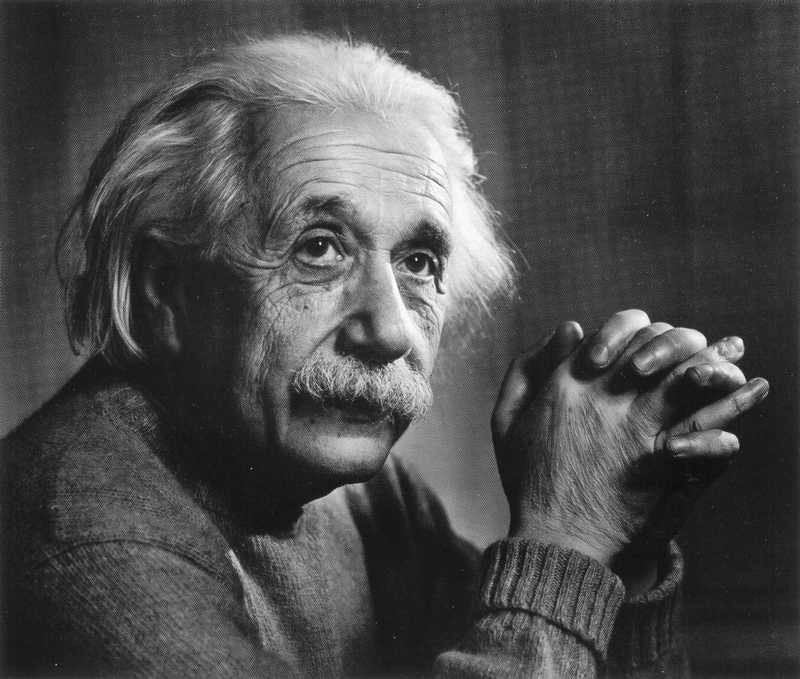
\includegraphics[height=3cm]{图2_5图2_6_a}
    \caption{}
    \label{图2_8_a}
  \end{subfigure}
  \hspace{4em}%
  \begin{subfigure}{0.2\textwidth}
    \includegraphics[height=3cm]{图2_8_b}
    \caption{}
    \label{图2_8_b}
  \end{subfigure}
  \hspace{4em}%
  \begin{subfigure}{0.25\textwidth}
    \includegraphics[height=3cm]{图2_8_c}
    \caption{}
    \label{图2_8_c}
  \end{subfigure}
  \caption{图像的幅度谱和相位谱。(a)原图像; (b)图像的幅度谱; (c)图像的相位谱。}
  \label{图2_8}
\end{figure}

幅度谱也是频率谱,它展示了一幅空间域的图像所对应的频率分布。频域下的每一点$(u,v)$的幅值$\Vert F(u,v)\Vert$用来表示该频率的正(余)弦波在叠加中所占的比例,决定了一幅图像中所包含的各种频率的分量大小,直接可以反应频率信息。相位谱相对幅度谱表面上看不是很直观,看不出它的重要性,它隐含的是傅里叶变换后的实部和虚部之间对应的某种比例关系,与图像的结构有密切的联系,相位谱决定了傅里叶变换的每一个频率分量分布在图像中的什么位置。可以大致的理解,图像的明暗对比度信息包含在幅度谱中,而图像的结构信息包含在相位谱中,可以通过实验说明二者各自的贡献。图~\ref{图2_9_b}是~\ref{图2_9_a}进行傅里叶逆变换时,通过将相位谱置零的方法消去相位谱信息,只保留幅度谱信息重建的图像,从图中已完全看不出原图的任何信息; 图~\ref{图2_9_c}是~\ref{图2_9_a}进行傅里叶反变换时,通过将幅度谱设置为某一定值消去幅度谱信息,单独保留相位谱信息重建的图像,从图像中基本上可以分辨出原图像大体的结构信息。为了进一步说明幅度谱和相位谱的作用,可以构造一个简单的例子。图~\ref{图2_10_a}、~\ref{图2_10_b}中分别是一张美女的图像和一张羊的图像,我们将这两幅图像的相位谱进行交换,即将美女的幅度谱加上羊的相位谱(如图~\ref{图2_10_c}),用羊的幅度谱加上美女的相位谱(如图~\ref{图2_10_d}),通过傅里叶反变换的公式得到重构后的图像,通过这个例子可以发现,经过交换相位谱和反变换后获得的图像信息与其相位谱所对应的信息是一致的。从以上两个简单的示例可以看出相位谱对于信号重建具有十分重要的作用,幅度的大小影响了图像的灰度信息,但是如果丢失了相位信息,整幅图像的结构和完整性则受到了严重的影响,这也是很多图像处理包括显著性检测经常只对图像变换后的幅度谱进行处理而保留图像相位谱的主要原因。
\begin{figure}[h]
  \centering%
  \begin{subfigure}{3cm}
    \includegraphics[height=3cm]{图2_9_a}
    \caption{}
    \label{图2_9_a}
  \end{subfigure}
  \hspace{4em}%
  \begin{subfigure}{0.2\textwidth}
    \includegraphics[height=3cm]{图2_9_b}
    \caption{}
    \label{图2_9_b}
  \end{subfigure}
  \hspace{4em}%
  \begin{subfigure}{0.25\textwidth}
    \includegraphics[height=3cm]{图2_9_c}
    \caption{}
    \label{图2_9_c}
  \end{subfigure}
  \caption{幅度谱和相位谱重建图像。(a)原图像; (b)幅度谱重建图; (c)相位谱重建图。}
  \label{图2_9}
\end{figure}
\begin{figure}[b]
  \centering%
  \begin{subfigure}{0.3\textwidth}
    \includegraphics[height=4cm]{图2_10_a}
    \caption{}
    \label{图2_10_a}
  \end{subfigure}
  \hspace{4em}%
  \begin{subfigure}{0.3\textwidth}
    \includegraphics[height=4cm]{图2_10_b}
    \caption{}
    \label{图2_10_b}
  \end{subfigure}
  \hspace{4em}%
  \begin{subfigure}{0.3\textwidth}
    \includegraphics[height=4cm]{图2_10_c}
    \caption{}
    \label{图2_10_c}
  \end{subfigure}
  \hspace{4em}%
  \begin{subfigure}{0.3\textwidth}
    \includegraphics[height=4cm]{图2_10_d}
    \caption{}
    \label{图2_10_d}
  \end{subfigure}
  \caption{幅度谱和相位谱的关系。(a)美女图像; (b)羊的图像; (c)美女幅度谱加羊相位谱; (d)羊幅度谱加美女相位谱。}
  \label{图2_10}
\end{figure}

在频域显著性检测中,主要是通过分析幅度谱和相位谱的特点,对变换得到的谱进行相应的处理,如对幅度谱进行滤波操作(低通滤波、中值滤波等),频率调频,利用剩余谱假设理论对幅度谱进行处理,或者直接将幅度谱去掉保留图像的相位谱进行傅里叶反变换获得图像的显著信息等方法。有关图像频域显著性检测方法将在第~\ref{cha3}章进行详细分析。

%=============================================================================================================
\section{后处理}
\label{2_4}

为了获得较好的显著性检测效果,在产生显著图后还需要进行进一步处理得到最终的显著图~\cite{BorjiTIP2013Quantitative}。正如SR模型~\cite{HouXiaodiCVPR2007Residual}所介绍的,通常经过傅立叶反变换后获得的显著图往往需要对图像中的每一个元素进行平方,然后将平方后的图像与一个合适的高斯滤波器进行滤波从而得到最终的显著图,进行平方的目的是提高图像的对比度,进行高斯滤波的目的~\cite{ZhangLiming2010Book}一方面为了抑制图像的噪声,另一方面为了提高显著性检测的效果。其表达式如下:
\begin{linenomath}
\begin{align}
SM(x,y)=g(x,y)\ast S(x,y)^{2}
\label{式2_37}
\end{align}
\end{linenomath}
其中,$S(x,y)$为反变换后的图像,$g(x,y)$为一个低通高斯滤波器,图~\ref{图2_11}表示将获得的显著图进行后续高斯滤波处理得到处理后的显著图,从图中可以明显看出,通过后续滤波处理,显著性区域得到了增强,而背景区域受到了抑制。为了进一步提高显著性检测结果,还可以进行其他的处理,如中央偏见设置(center-bias setting)、边缘切割(border cut)等。
\begin{figure}[h] % use float package if you want it here
  \centering
  \includegraphics[height=7.5cm]{图2_11}
  \caption{显著性检测后处理的高斯滤波效果图。上面是显著图,下面是对显著图进行高斯滤波处理的最终显著图。}
  \label{图2_11}
\end{figure}

以前的一些文献通过证明认为靠近图像中心的物体更能够引起人们产生视觉注意~\cite{JuddICCV2009Learning},这个研究说明靠近图像中央的区域要比远离图像中央的区域更显著,并通过实验说明了这种显著性分布可以简单有效的模拟为高斯分布~\cite{ZhangLin2013SDSP},这个理论即为中央偏见。在进行高斯偏见设置时,将图像进行高斯权限设置,即由中心向四周位置分布的元素乘以高斯分布中所对应的值,最后进行归一化处理得到显著图。边缘切割(border cut)是指在进行显著性检测后处理中将图像的边缘设置成一定像素的窄边区域,这样做的目的是当滤波器位于图像的边缘,滤波响应不能够被很好的定义,并且可以避免边界区域收敛速度慢的缺点~\cite{ChengMingMingCVPR2011Global}。

%=============================================================================================================
\section{评价方法}
\label{2_5}

为了测试显著性检测方法的准确性、客观比较各种不同的方法,需要对方法进行评价。显著性检测可以分为注视焦点预测和显著性区域检测\cite{LiYinCVPR2014Secrets},针对不同的分类选择不同的评价方法。显著性检测的数据集需要人工标记获得真实数据(ground-truth),$1$表示显著性区域,$0$表示非显著性区域,从最终显著图中提取显著目标可以选择全局阈值分割方法,即将阈值从0逐步增加至255,利用没一个阈值对显著图进行分割,或对显著图进行自适应阈值分割处理~\cite{AchantaCVPR2009Frequency},然后将计算得到的显著图进行定性定量分析,选择合适的评价方法,如精度-召回率曲线(PR曲线)、受试者工作特征曲线(ROC曲线)、F-测量值(F-measure值)或AUC值等。下面将介绍几种显著性检测评价方法。

%-------------------------------------------------------------------------------------------------------------
\subsection{PR曲线和ROC曲线}
\label{2_5_1}

对于分类模型的两类问题,输出可以分为阳性或阴性~\cite{Powers2007Evaluation}。在双分类器分类中可能会得到$4$类结果:如果预测的是阳性,真实的也是阳性(TP),那么此时就叫作真阳性; 如果预测的是阳性,而真实的为阴性,则此时就叫做假阳性(FP); 相反,如果预测的和真实的都是阴性,那么这叫作真阴性(TN); 如果预测的为阴性,真实的为阳性,这时候就称作假阴性(FN),可以通过下面的表格~\ref{图2_12}来表示:
\begin{figure}[h] % use float package if you want it here
  \centering
  \includegraphics[height=5.5cm]{图2_12}
  \caption{双分类器中的四种分类结果值}
  \label{图2_12}
\end{figure}
在讨论PR曲线和ROC曲线时往往离不开下面的表格图。

PR曲线是指查准率-查全率曲线,在PR空间中,$x$坐标为召回率值(recall),y轴代表精度值(precision),二者分别定义为:
\begin{linenomath}
\begin{align}
\textrm{Recall =$\frac{TP}{TP+FN}$}\label{式2_38}\\
\textrm{precision =$\frac{TP}{TP+FP}$}\label{式2_39}
\end{align}
\end{linenomath}

ROC曲线是用来描述灵敏度的曲线,可以通过计算真阳性率和假阳性率来实现。在ROC空间中,$x$坐标是假阳性率值,$y$坐标代表真阳性率值,二者分别定义如下:
\begin{linenomath}
\begin{align}
\textrm{FalsePositiveRate =$\frac{FP}{FP+TN}$}\label{式2_40}\\
\textrm{TruePositiveRate =$\frac{TP}{TP+FN}$}\label{式2_41}
\end{align}
\end{linenomath}

在进行计算时,可以通过对显著图调整不同的阈值,然后与真实数据结合得到不同的PR值(或ROC值),从而可以得到一条曲线。对于PR曲线,显然查的既准又全的比较好,即越靠近坐标$(1,1)$的位置越好; 对于ROC曲线,显然真阳性率越大、假阳性率越小越好,即越靠近坐标$(0,1)$的位置越好。图~\ref{图2_13}分别给出了PR曲线和ROC曲线。
\begin{figure}[h]
  \centering%
  \begin{subfigure}{0.4\textwidth}
    \includegraphics[height=5cm]{图2_13_a}
    \caption{}
    \label{图2_13_a}
  \end{subfigure}
  \hspace{4em}%\\\\
  \begin{subfigure}{0.4\textwidth}
    \includegraphics[height=5cm]{图2_13_b}
    \caption{}
    \label{图2_13_b}
  \end{subfigure}
  \caption{PR曲线和ROC曲线图。(a)PR曲线; (b)ROC曲线。}
  \label{图2_13}
\end{figure}

%-------------------------------------------------------------------------------------------------------------
\subsection{AUC值}
\label{2_5_2}

为了更好的说明ROC表达结果的好坏,AUC被提了出来,简单的说AUC就是ROC曲线下的面积~\cite{Green1966book},在了解了ROC曲线的构造之后,显然AUC的数值不能大于$1$,而由于ROC曲线一般都处于$y=x$这条直线上,因此它的取值范围会在$0.5$到$1$之间。用AUC作评价标准的原因是大多数情况下ROC曲线并不能比较清晰的说明分类效果的好坏,而AUC作为数值则能更好的说明哪个分类器的效果更好。在显著性检测评价的情况下,人眼注视的点被看作阳性集合,从其他位置采样获得的点被看作阴性集合~\cite{Tatler2005correlates}。同PR曲线和ROC曲线介绍显著性效果评价类似,显著图可以被看作二值分类,通过阈值分割提取出阳性样本,从而得到真阳性率值和假阳性率值,画出ROC曲线,然后计算每一幅图像ROC曲线下的面积,最后通过计算整个数据集的平均值得到最终的AUC值。对于越好的注视结果预测,它所对应的AUC的值越接近$1$。

%-------------------------------------------------------------------------------------------------------------
\subsection{KL散度}
\label{2_5_3}

KL用来度量两个概率分布P和Q的差别,在典型情况下,P代表数据的真实分布,Q代表数据的理论分布。在显著性检测的情况下,它可以衡量注意焦点位置的视觉显著性度量直方图和随机位置的视觉显著性度量直方图之间的散度~\cite{Kullback1959book,IttiCVPR2005principled}。如果一个显著性检测模型可以比较好的预测人类的注意焦点,在注意焦点的显著性度量就会大大高于随机选取的位置点,KL的值就会比较高。因此,KL的值越高,说明显著性检测模型越好。在进行计算显著性度量的直方图之间KL散度的时候,选取的两种直方图分别是场景图像中注意焦点位置的显著性直方图和数据库中随机选择的场景中同一位置的显著性直方图。将测试图像的显著性分为$10$个区间,统计出该图像所有注意焦点落在每个区间的次数,然后除以总的注视点数,得到该幅图像在注意焦点处的显著性直方图,然后对测试集中的每幅图像进行如上的操作,再进行均值化处理,最后得到注意焦点处的显著性直方图。

对于随机点的选取方式,可以在同一点位置,不同的显著图中进行选取,取多次后再取均值。KL距离的公式为:
\begin{linenomath}
\begin{align}
D_{KL}=\sum_{i}P(radom(i))*log(\frac{P(random(i))}{P(fixation(i))})
\label{式2_42}
\end{align}
\end{linenomath}
公式中$i$等于显著性区间的个数,对得到的$D_{KL}$的值进行平均,从而获得最终的KL散度值。

%-------------------------------------------------------------------------------------------------------------
\subsection{线性相关系数(CC)}
\label{2_5_4}

线性相关系数在图像处理中常用来比较两幅图像的之间的关系,其广泛应用在图像配准、目标识别和视差测量中。线性相关系数衡量变量之间的关系强度,在显著性检测中亦可以用来衡量两幅显著图之间的线性强度关系~\cite{Jost2005Assessing}。线性相关系数的定义如下:
\begin{linenomath}
\begin{align}
CC(G,S)=\frac{\sum_{x,y}(G(x,y)-\mu_{G})\cdot(S(x,y)-\mu_{S})}{\sqrt{\sigma_{G}^{2}\cdot\sigma_{S}^{2}}}
\label{式2_43}
\end{align}
\end{linenomath}
其中,$\mu_{G}$和$\mu_{S}$分别是$G$和$S$的均值,$\sigma_{G}^{2}$和$\sigma_{S}^{2}$分别代表$G$和$S$的方差。选择线性相关系数的优势在于它可以通过$-1$到$+1$之间的单个标量值对比两个变量之间的相关性,当相关系数值越接近于$+1$或$-1$时,说明它们之间的相关性越强。

%-------------------------------------------------------------------------------------------------------------
\section{本章小结}
\label{2_5_5}

本章详细介绍了频域显著性检测方法的一般步骤,该方法具有计算简单、快速的特点。频域显著性检测算法首先进行预处理,提取图像的底层特征,常见的是将图像进行颜色空间的转换,如转换到RGB空间、Lab空间或IRGBY空间等,然后进行图像的变换,最常见的是傅里叶变换,将图像从空间域转换到频域,还有其他的转换方法,如离散余弦变换、小波变换等,图像转换到频域后,通过分析图像对应的谱在频域的分布特点从而进行相应的频域处理,处理完再通过傅里叶反变换转换到空间域,最后通过后处理机制对显著图进行进一步增强得到最终的显著图。为了比较显著效果的好坏,我们还介绍了一些比较常用的显著性评价方法,如PR曲线、ROC曲线、AUC值和CC值等,这些评价方法保证了显著性检测方法的客观性和准确性。


\chapter{频域显著性检测模型}
\label{cha3}

在上一个章,我们主要对频域显著性检测的一般处理步骤进行了详细的说明,对图像频率谱进行了简单的分析。本章将对国内外典型的频域显著性检测模型进行详细的介绍,尤其是对图像转换到频域进行的谱处理进行具体分析。
%=============================================================================================================
\section{谱剩余显著性检测模型(SR)}
\label{3_1}

2006年,侯晓迪首次提出了一种既简单又快速的频域显著性检测算法---谱剩余算法(SR)~\cite{HouXiaodiCVPR2007Residual}。SR方法从信息论\cite{Barlow1961Possible}的观点认为在一幅图像或一个场景中所有的信息被分做两部分,一部分是图像的新颖部分代表显著性信息,另一部分是图像的冗余部分代表非显著性信息或先验信息,即:
\begin{equation}
H(Image)=H(Innovation)+H(Prior Knowledge)
\label{式3_1}
\end{equation}
根据有效编码理论,图像的冗余信息应该被抑制掉而保留图像的新颖部分。对于一幅图像如何去将这两种信息进行区分呢? 直观的理解认为,属于新颖部分像素的统计特性低于冗余部分的像素。自然图像统计的不变特性中,尺度不变性\cite{Ruderman1994Statistics,Srivastava2003Advances}被认为是最著名最广泛的一种属性,又称作$1/f$法则,其表达式如下:
\begin{equation}
E\{A(f)\}\propto 1/f
\label{式3_2}
\end{equation}
$A(f)$表示图像进行傅里叶变换后的幅度谱,$E\{\}$表示数学期望。它说明自然图像傅里叶变换的幅度谱是有规律的。图~\ref{图3_1}显示了不同图像的对数幅度谱,从图中可以看出不同图像所对应的曲线具有相似的形状,这种相似性说明了自然图像的冗余所在。如果对多幅图像的对数幅度谱进行平均处理,从图~\ref{图3_2}可以发现,处理后的曲线比较平滑,这说明了均值对数幅度谱具有局部线性的特征\cite{HouXiaodiCVPR2007Residual}。
\begin{figure}[!t] %插图
\centering
\includegraphics[width=0.8\textwidth]{图3_1}
\caption{自然图像及其对数幅度谱曲线~\cite{HouXiaodiCVPR2007Residual}}
\label{图3_1}
\end{figure}
\begin{figure}[!t] %插图
\centering
\includegraphics[width=0.8\textwidth]{图3_2}
\caption{不同图像的均值对数幅度谱曲线~\cite{HouXiaodiCVPR2007Residual},自左至右分别是1幅、10幅、100幅。}
\label{图3_2}
\end{figure}

视觉系统会将图像的冗余信息去除,因此从自然图像的幅度谱中减去冗余信息的幅度谱,剩下的即为显著部分的幅度谱,这就是谱剩余的方法,所以对于自然图像,能够引起感兴趣产生视觉注意的是对数幅度谱中异常的信息,用$\mathcal{R}(f)$来表示,则:
\begin{equation}
H(\mathcal{R}(f))=H(\mathcal{L}(f)|\mathcal{A}(f))
\label{式3_3}
\end{equation}
其中,$\mathcal{L}(f)$表示自然图像的对数幅度谱,先验信息$\mathcal{A}(f)$表示一般对数幅度谱,图~\ref{图3_2}已经说明一般对数幅度谱拥有局部线性的特征,因此,可以用一个$n \times n$局部均值滤波器${h}_{n}(f)$对对数幅度谱进行滤波得到一般对数幅度谱$\mathcal{A}(f)$:
\begin{equation}
\mathcal{A}(f)={h}_{n}(f)\ast \mathcal{L}(f)
\label{式3_4}
\end{equation}
因此,剩余谱$\mathcal{R}(f)$可以表示为:
\begin{equation}
\mathcal{R}(f)=\mathcal{L}(f)-\mathcal{A}(f)
\label{式3_5}
\end{equation}
最后,将取得的剩余谱与初始图像的相位谱结合进行傅里叶反变换获得显著图。该算法可以归纳如下:
\begin{linenomath}
\begin{align}
\mathcal{A}(f) &= \Re(\mathfrak{F}[\mathcal{I}(x)])\label{式3_6}\\
\mathcal{P}(f) &= \Im(\mathfrak{F}[\mathcal{I}(x)])\label{式3_7}\\
\mathcal{L}(f) &= log(\mathcal{A}(f))\label{式3_8}\\
\mathcal{R}(f) &= \mathcal{L}(f)-h_{n}(f)\ast \mathcal{L}(f) \label{式3_9}\\
\mathcal{S}(x) &= g(x)\ast \mathfrak{F}^{-1}[exp(\mathcal{R}(f)+\mathcal{P}(f))]^{2}\label{式3_10}
\end{align}
\end{linenomath}
其中,$\mathfrak{F}$和$\mathfrak{F}^{-1}$分别代表傅里叶变换和傅立叶反变换,$\mathcal{P}(f)$代表原图像的相位谱,$\Re$与$\Im$分别表示傅里叶变换得到的的实部和虚部,$g(x)$是高斯滤波器用于提高图像的显著性效果。

%=============================================================================================================
\section{相位谱四元傅里叶变换显著性检测模型(PQFT)}
\label{3_2}

尽管剩余谱算法~\cite{HouXiaodiCVPR2007Residual}既快又简单,而且能够得到较好的显著性检测结果,但是它的原因却是不明了的,而且不能确定幅度谱中的剩余谱是否真正反映了一个场景中的新颖部分或是显著区域,如图~\ref{图3_3},(a)和(c)是具有相同背景,但是图(a)有黄色头饰(显著性目标),图(c)中黄色头饰在前景中消失了,这两幅图像所对应的对数幅度谱分别为(b)和(d)。很明显,尽管这两幅图像所对应的幅度谱有微小的区别,但是很难从这两种曲线中区分图像新颖的信息(显著性物体)是什么。另外,谱剩余算法中只使用了图像的灰度信息,并没有考虑颜色等因素的影响,所以对于颜色特征区别明显而亮度变化不明显的图像该种算法效果不好。
\begin{figure}[!t] %插图
\centering
\includegraphics[width=0.8\textwidth]{图3_3.png}
\caption{场景中有无黄色头饰(显著性物体)的两幅幅度谱曲线图的对比}
\label{图3_3}
\end{figure}

基于以上分析,Guo等人在谱剩余算法的基础上提出了相位谱四元傅里叶变换算法(PQFT)~\cite{GuoChenleiCVPR2008Spatio}。在SR模型中,相位谱在计算的过程中被完整的保留了下来。因此,在PFT算法中,忽略剩余谱的处理过程,直接去掉幅度谱,只使用相位谱进行傅里叶反变换,就可以得到空间域的显著图。如图~\ref{图3_4}所示,给出一个矩形脉冲的波形,忽略幅度谱进行傅里叶反变换后,在脉冲的边缘处会产生巨大的尖峰,这是因为在脉冲的边缘是由无数的正弦函数叠加而成的; 当对于一个单一频率的正弦波后,去掉幅度谱的反变换的信号则没有明显的尖刺。
\begin{figure}[!t] %插图
\centering
\includegraphics[width=0.8\textwidth]{图3_4}
\caption{一维信号与对应信号相位谱的反变换示意图。左边是原始信号,右边是左边信号仅利用相位谱进行傅里叶反变换的重构图。}
\label{图3_4}
\end{figure}

输入一幅图像$I(x,y)$,PFT具体的处理过程如下:
\begin{linenomath}
\begin{align}
f(x,y) &= F(I(x,y))\label{式3_11}\\
p(x,y) &= P(f(x,y))\label{式3_12}\\
sM(x,y) &= g(x,y)\ast\Vert F^{-1}[e^{i\cdot p(x,y)}]\Vert^{2}\label{式3_13}
\end{align}
\end{linenomath}
其中,$F()$代表傅里叶变换,$P()$代表取傅里叶变换的相位谱,$F^{-1}[]$为傅里叶反变换,$g(x,y)$为高斯滤波器用于提高图像的显著性效果。通过实验可以证明,该方法与谱剩余方法获得的显著图几乎一样,因此也证明了剩余谱不是产生显著性的必要条件,并且PFT方法更加迅速简单。

之后,Guo等人~\cite{GuoChenleiCVPR2008Spatio}对PFT方法进行了进一步扩展,他们增加了图像的颜色特征$RG$和$BY$,并且加入了运动特征$M$,于是将图像的四个特征图用四元数表示出来,利用四元数傅里叶变换将图像转换到频域,然后将频域中的幅度谱去掉,再进行四元数傅里叶反变换转换到空间域得到最终的显著图。

%=============================================================================================================
\section{频域除法归一化显著性检测模型(FDN)}
\label{3_3}

除法归一化~\cite{BianCognNeurodyn2010Visual}可以用来模仿视觉神经细胞的侧抑制机制,它被看作是对视觉注意起关键作用的中心--周围对抗机制。在谱白化理论~\cite{Bian2009Biological}的基础上,频域除法归一化是一种基于频域、具有生物学依据,并且符合信息理论的自底向上的视觉注意显著性检测算法。该种方法首先证明了频域方法也具有生物学依据,认为视觉神经节细胞和V1区的简单细胞的特征提取,在频域中可以近似的表示为在图像频谱上用分割的带通滤波相乘。除法归一化是指对于每个具有相同种类特征的简单细胞的输出,除法归一化的输出等于每个像素输出除以其周围像素的输出加权和加上一个常数,除法归一化模型定义为:
\begin{linenomath}
\begin{align}
\hat{r}_{i}[n]=\frac{r_{i}[n]}{\sqrt{\sum_{n'}w[n']|r_{i}[n']|^{2}+\sigma^{2}}}
\label{式3_14}
\end{align}
\end{linenomath}
其中$r_{i}[n']$是$r_{i}[n]$周围的输出,$w$是权值矩阵,$\sigma$是一个常数。频域除法归一化的处理步骤如下:
\begin{enumerate}
\item 变换图像尺寸并将自然图像从RGB彩色空间转到Lab彩色空间,然后将图像分为3通道:$s_{c}|c\in\{l,a,b\}$;
\item 取每个通道$s$进行傅里叶变换:
\begin{linenomath}
\begin{align}
S[k]=\sum_{x}s(x)e^{-2\pi kx/N}
\label{式3_15}
\end{align}
\end{linenomath}
\item 利用频域分解方法把每个傅里叶系数$k$归到一个特征$i$;
\item 计算每个特征$i$的除法归一化分母$E_{i}$,该文献中将两个归一化参数$w$和$\sigma$都设置为1:
\begin{linenomath}
\begin{align}
E_{i}=\sqrt{w\sum_{k\in i}|S[k]|^{2}/N+\sigma^{2}}
\label{式3_16}
\end{align}
\end{linenomath}
\item 创建分母图$E[k]$:$E[k]=\{E_{i}\in i\}$
\item 计算频域除法归一化的结果值:
\begin{linenomath}
\begin{align}
\hat{S}[k]=\frac{S[k]}{E[k]}
\label{式3_17}
\end{align}
\end{linenomath}
\item 取每个频谱$\hat{S}$的傅里叶反变换:
\begin{linenomath}
\begin{align}
\hat{s}(x)=W(x)|\sum_{k}\hat{S}[k]e^{2\pi kx/N}|^{2}
\label{式3_18}
\end{align}
\end{linenomath}
\item 最后从所有通道$c$中求出最终的显著图$sM$:
\begin{linenomath}
\begin{align}
sM(x)=max\{\hat{s}_{c}(x)\}
\label{式3_19}
\end{align}
\end{linenomath}
\item 利用高斯滤波器对显著图进行平滑处理。
\end{enumerate}

%=============================================================================================================
\section{基于相位谱和调谐幅度谱的显著性检测模型(PTA)}
\label{3_4}

针对谱剩余算法得到的显著图对比度比较差、细节显著性检测结果不太理想的问题,李崇飞等人~\cite{李崇飞2012相位谱}经过分析图像频谱特点和显著性的关系,提出了一种基于频谱分析的显著性区域检测方法。该算法分析了图像数据进行傅里叶变换之后,显著信息和非显著信息都会以统计信息的方式保留在傅里叶变换的频谱中,通过证明相位谱对于图像显著信息的重要意义,该方法保留了相位谱,然后该文献在分析了幅度谱中冗余信息和显著信息的统计特性后,提出了幅度谱分段调谐的方法,即抑制幅度谱的高频分量,增强幅度谱的低频分量,达到抑制图像大部分冗余信息并且保留并增强图像的显著性信息的效果。

PTA方法~\cite{李崇飞2012相位谱}认为幅度谱是各种基波的加权和,非显著性信息的幅值(比重比较大)在幅度谱中表现为比较高的幅值,需要对它们进行抑制; 而代表显著信息的幅值(比重比较小)在幅度谱中表现为比较低的幅值,需要对它们进行保留和增强。PTA~\cite{李崇飞2012相位谱}通过利用阈值的方法确定了显著性特征和非显著性特征在频域幅度谱的分界(边界),自适应抑制了大于阈值的幅度谱,自适应增强了小于阈值的幅度谱,从而突出了显著性特征。对于幅度谱$a(u,v)$显著性分类阈值$\Delta$为:
\begin{linenomath}
\begin{align}
\Delta=\gamma M(a(u,v))
\label{式3_20}
\end{align}
\end{linenomath}
幅度谱调谐$a'(u,v)$为:
\begin{linenomath}
\begin{align}
a'(u,v) = \left\{ \begin{array}{ll}
f(u,v)/(|a(u,v)-\Delta|^{\alpha}) & a(u,v)>\Delta\\
f(u,v)|a(u,v)-\Delta|^{\beta}) & a(u,v)\leq \Delta
\end{array} \right.
\label{式3_21}
\end{align}
\end{linenomath}
其中,$f(u,v)$为图像傅里叶变换后的值,$\alpha$和$\beta$为参数,依据图像的对比度通过实验进行选择,一般如果图像的对比度比较大时,即像素方差较大,则$\alpha$取值比较大而$\beta$的值较小,反之则$\alpha$取值比较小而$\beta$的值较大。给定一幅图像$I(x,y)$,算法的结构如下:
\begin{linenomath}
\begin{align}
f(u,v) &= F(I(x,y))\label{式3_22}\\
p(u,v) &= P(f(u,v))\label{式3_23}\\
a(u,v) &= \Vert f(u,v)\Vert \label{24}\\
I'(x,y) &= \Vert F^{-1}[exp(log(a'(u,v)+i\cdot p(u,v)))]\Vert^{2}\label{式3_25}\\
S(x,y) &= G\ast I'(x,y)\label{式3_26}
\end{align}
\end{linenomath}

基于相位谱和调谐幅度谱的显著性检测方法在显著图对比度和显著性细节检测等方面比谱剩余方法的性能效果有了更大的提升。

%=============================================================================================================
\section{基于图像签名的显著性检测模型(SIG)}
\label{3_5}
图像签名~\cite{HouXiaodiTPAMI2012Signature}是由侯晓迪等人最早提出的,它在整个频域范围内丢弃了信号的幅度谱信息,仅仅保留了图像的离散余弦变换部分的符号,即保留了图像的相位谱。在~\cite{Hou2014Phd}中已经被证明了图像重要的视觉信息主要保留在幅度谱中。该描述符是基于信号的稀疏性理论提出的,近年来稀疏性理论已被广泛的应用在数字信号和计算机视觉等领域,图像稀疏性理论认为,图像都是稀疏的。信号经过稀疏变换后,绝大多数有用的信息都将集中分布在少量的变换系数中~\cite{郑源彩2012稀疏},常见的图像稀疏变换的方法有小波变换、离散余弦变换和有限差分等,图像签名即采用的离散余弦变换。图像签名的定义为:
\begin{linenomath}
\begin{align}
\textrm{ImageSignature$(x)$=sign$DCT(x)$}
\label{式3_27}
\end{align}
\end{linenomath}

侯晓迪~\cite{HouXiaodiTPAMI2012Signature}证明了图像签名可以用来粗略的获得图像前景的位置,并且提出了两个命题:
\begin{enumerate}
\item 图像签名的重构图像可以用来从稀疏背景中估计图像稀疏性的前景位置,即图像签名可以抑制图像的背景;
\item 对于一个非零元素的前景信号$f$,通过图像签名重构后的信号有$79\%$的信息保留在前景信号中。
\end{enumerate}
其证明过程如图~\ref{图3_5}所示,给定一幅图像$f$,它可以分为前景信号$f$和背景信号$b$,即
\begin{linenomath}
\begin{align}
x=f+b&&x,f,b\in\mathbb{R}^{N}
\label{式3_28}
\end{align}
\end{linenomath}
$f$经过离散余弦变换可以得到变换后的前景$\hat{f}$,背景$b$经过离散余弦变换可以得到变换后的背景$\hat{b}$,通过相加可以得到离散余弦变换后的信号$\hat{x}$,对$\hat{x}$取符号运算即可得到信号的图像签名。根据上述命题1的理论,此时信号$\hat{x}$的符号值与离散余弦变换的前景$\hat{f}$的符号值是相近的,因为前景信号$f$和离散余弦变换背景信号$\hat{b}$都只有很少数量的非零分量。将$sign(\hat{f})$进行离散余弦反变换得到重构信号$\bar{f}$,然后根据上述命题2可得,重构后的信号$\bar{f}$与前景信号$f$是近似的,进而有$\bar{x}$近似等同于$f$,从而证明了图像签名可以用来粗略的获得图像前景的位置,并可以近似估计前景的大小。
\begin{figure}[h] %插图
\centering
\includegraphics[width=0.8\textwidth]{图3_5}
\caption{图像签名的证明框架~\cite{HouXiaodiTPAMI2012Signature}}
\label{图3_5}
\end{figure}

利用图像签名算子重构后的图像可以检测空间中嵌入在稀疏背景中的前景信号,重构后的信号与人类感兴趣(产生视觉注意)的区域是重叠的,因此可以用来进行图像的显著性检测。给定图像$x$,rgb-SIG显著性检测算法如下:
\begin{enumerate}
\item 输入图像$x$,将图像的大小转换为一定的大小,并提取图像的R、G和B颜色特征$x^{i} (i=1,2,3)$;
\item 取每个通道$x^{i}$进行离散余弦变换,再求$sign$值:
\begin{linenomath}
\begin{align}
\textrm{ImageSignature$(x^{i})$=sign$(DCT(x^{i}))$}
\label{式3_29}
\end{align}
\end{linenomath}
\item 对变换后的图像进行离散余弦反变换重构:
\begin{linenomath}
\begin{align}
\bar{x^{i}}=IDCT[sign((DCT(x^{i})))]
\label{式3_30}
\end{align}
\end{linenomath}
\item 利用高斯滤波对显著图进行处理:
\begin{linenomath}
\begin{align}
m=g\ast\sum_{i}(\bar{x}^{i}\circ\bar{x}^{i})
\label{式3_31}
\end{align}
\end{linenomath}
\item 最后对$m$取均值获得最终的显著图。
\end{enumerate}

值得注意的是,图像签名是计算机视觉领域中的一个简单有力的算子,可以用来估计图像前景的位置和尺寸的大小,显著性检测是该算子的一个具体应用,在后面本文的算法中也会用到图像签名算子。

%=============================================================================================================
\section{基于频域尺度空间分析的显著性检测模型(HFT)}
\label{3_6}

显著性目标往往是独特和不规则的,这些特征很容易与周围背景区分开来,很多算法是通过检测图像的显著性计算的。基于频域尺度空间分析的显著性检测方法~\cite{LiJianTPAMI2013Scale}并没有试图寻找独特不规则的显著性目标,而是通过分析非显著性区域的规则特性在频域中的表现,进而抑制非显著性区域来进行显著性检测。

该模型假设自然图像是由显著性区域和所谓的规则的非显著性区域构成的,而非显著性区域表现为重复性模式,通过傅里叶变换的幅度谱可知,规则的非显著性区域在幅度谱上表现为尖峰,并且重复的模式越多尖峰越明显。因此,为了抑制非显著性区域,可以通过抑制幅度谱中的尖峰进行处理。该模型通过利用高斯滤波器在合适尺度上对幅度谱进行平滑操作,从而在空间域中抑制了重复模式。不同的滤波尺度对检测显著性的要求不一样,小的滤波尺度可以用来检测大的显著性区域,大的滤波尺度可以用来检测小的显著性区域。

为了解决尺度选择的问题,HFT模型提出了谱尺度空间(SSS)~\cite{LiJianTPAMI2013Scale},即通过一系列的高斯滤波簇对图像的幅度谱进行滤波,得到一系列滤波后的幅度谱。给定一幅图像的幅度谱$A(u,v)$,谱尺度空间是将$A(u,v)$与一系列的高斯核卷积获得的衍生信号$\Lambda$。选择的高斯滤波簇为:
\begin{linenomath}
\begin{align}
g(u,v;k)=\frac{1}{\sqrt{2\pi}2^{k-1}t_{0}}e^{(u^2+v^2)/(2^{2k-1}t_{0}^{2})}
\label{式3_32}
\end{align}
\end{linenomath}
其中$k$是尺度参数,$k=1,\dots,K$,$K$与图像的尺寸有关:$K=[log_{2}min\{H,W\}]+1$,$H$和$W$分别是图像的高度和宽度。$t_{0}$为一个参数。因此,尺度空间定义为:
\begin{linenomath}
\begin{align}
\Lambda(u,v;k)=(g(.,.;k)\ast A)(u,v)
\label{式3_33}
\end{align}
\end{linenomath}

通过计算得到图像的尺度空间,然后与图像的相位谱(相位谱不变)进行傅里叶反变换进而获得一系列显著图,如何对这些生成的显著图进行选择呢?HFT模型提出了运用图像熵的方法选出效果较好的显著图作为最终的显著图。图像熵~\cite{Abutaleb1989Automatic}用来统计图像的特征,主要反映了图像平均信息量的多少,表征图像灰度分布的聚集特性。灰度图像的一元灰度熵为:
\begin{linenomath}
\begin{align}
H=\sum_{i=0}{255}p_{i}log p_{i}
\label{式3_34}
\end{align}
\end{linenomath}
其中$p_{i}$是某个灰度值在图像中出现的概率,该值可以通过图像直方图取得。尽管图像一维熵可以用来反映灰度分布的聚集特性,但是不能够反映灰度空间分布特性。为了表示该特征,HFT模型引入了图像二维熵,它是通过选择图像的邻域灰度值来作为灰度值分布的空间几何特征值,该模型进行了简单的处理,将图像的一维熵分布变量值$x$与高斯滤波器$g_{n}$进行卷积得到新的二维熵$H_{2D}$:$H_{2D}(x)=H\{g_{n}\star x\}$。二维熵可以表示图像中像素的位置灰度信息与邻域内灰度值分布信息的综合特性。HFT模型认为,二维熵值越小,图像的显著性效果越好,该模型选取了熵值最小的显著图作为最终的显著图。给定尺寸为$m×n$的图像$C$,基于频域尺度空间分析的显著性检测算法结构如下:
\begin{enumerate}
\item 提取图像的特征图$\{I,RG,BY\}$;
\item 根据图像的特征图,计算图像的四元傅里叶变换,获得图像的幅度谱$A$,相位谱$P$和特征轴谱$\chi$;
\item 利用高斯滤波簇对图像的幅度谱进行平滑滤波得到图像的尺度空间$\{\Lambda\}$;
\item 通过四元数傅里叶反变换将尺度空间中的衍生幅度谱与图像的相位谱反变换到空间域,得到一系列显著图;
\item 利用图像的二维熵选择合适的显著图作为最终的显著图$S$。
\end{enumerate}

%=============================================================================================================
\section{本章小结}
\label{3_7}

本章我们介绍了国内外几种典型的频域显著性检测算法,包括SR模型、PQFT模型、FDN模型、PTA模型、SIG模型和HFT模型,分别对他们提出动机、算法描述和表示意义上进行了详细的解释和说明。

%%% Local Variables: 
%%% mode: latex
%%% TeX-master: t
%%% End: 

\chapter{基于幅度谱分析的视觉显著目标检测模型(AA)}
\label{cha4}

通过上一章的分析我们知道,谱剩余算法~\cite{HouXiaodiCVPR2007Residual}和相位谱傅里叶变换算法~\cite{GuoChenleiCVPR2008Spatio}在一定程度上等价于一个梯度算子与高斯后续处理的结合。这是因为自然图像的幅度谱在低频区域的幅度值远远高于在高频区域的幅度值。如图~\ref{图4_1}所示,原图像的幅度谱绝大部分集中在低频区域,经过谱剩余处理后,(b)的幅度谱值比较均匀,高频区域的幅度谱和低频区域的幅度谱相差不大,这就类似等同于高频区域和低频区域分布量几乎相等,而傅里叶变换相位谱算法的处理则是将整个幅度谱设为同一个值,即将幅度谱处理为一个平面,这种处理换句话说就是抑制了幅度谱的低频区域,增强了幅度谱的高频区域。基于以上的分析可知,通过傅里叶反变换可以看出谱剩余算法和相位谱傅里叶变换算法获得的显著图几乎一样,检测的都是图像的边缘和纹理密集的区域,这也说明了他们的算法仅仅可以用来检测中央周围对比度比较强烈的小的显著区域,对于大的显著区域的检测则比较困难。
\begin{figure}[h]
  \centering
  \includegraphics[height=9.8cm]{图4_1}
  \caption{SR算法和PQFT算法与原图像频域变换及显著图的对比示意图。(a)是原始图像的变换; (b)是SR模型的变换; (c)是PQFT模型的变换。第一列:原图像; 第二列:频谱图; 第三列:对频谱图取log后的对数幅度谱图; 第四列:反变换后的图像。}
  \label{图4_1}    
\end{figure}

对于一个比较好的显著目标检测方法,其应该具备以下特点~\cite{AchantaCVPR2009Frequency}:
\begin{enumerate}
\item 小的显著目标和大的显著目标都可以检测;
\item 可以均匀的突出整个显著目标,而不仅仅突出目标的边缘或纹理较密集的区域;
\item 可以将显著目标从复杂的背景中检测出来;
\item 检测效率高,具有高效的图像处理能力,适应工程性应用。
\end{enumerate}

谱剩余算法和傅里叶变换相位谱算法以及在上一章节中介绍的其他算法不能同时满足上述所有的特点,如谱剩余算法~\cite{HouXiaodiCVPR2007Residual}和傅里叶变换相位谱算法~\cite{GuoChenleiCVPR2008Spatio}满足第3项和第4项特点,不满足第1、2项; PTA方法~\cite{李崇飞2012相位谱}满足1、3、4项,不满足第2项等。我们受到了SSS方法~\cite{LiJianTPAMI2013Scale}的启发,经过仔细的分析和实验,提出了一种新的频域显著性处理方法,通过与其他频域算法的对比,我们的方法可以获得更好的显著目标检测效果。

%=============================================================================================================
\section{幅度谱分析}
\label{4_1}

根据第~\ref{cha2}章的分析可知,图像通过傅里叶变换后,信息都将保留在变换后的幅度谱和相位谱中,幅度谱代表了图像的明暗对比度信息,而图像的结构信息包含在相位谱中,因此图像的相位谱在变换中是不能进行改变的,要保留下来,图像频域显著性检测主要是对信号的幅度谱进行处理。

%-------------------------------------------------------------------------------------------------------------
\subsection{图像中显著与非显著特性分析}
\label{4_1_1}

根据Li等人~\cite{LiJianTPAMI2013Scale}提出的观点,给定一幅图像,它可以被看作是由不同的小区域组成,而每个小区域可以称为一种模式。图~\ref{图4_2}是中国海洋大学作宣传片时用的图片(美丽的海洋),从所给的图像中我们可以看出图像被分成了不同的小区域,很多分块的小区域是非常相似的,或者说是重复区域,例如分块的海洋小区域,而海洋上的小岛分块之后,他们的小区域是不重复或独特的。根据视觉注意机制,反复出现的重复模式一般不会引起人类产生视觉注意,而异常或不重复出现的模式常常引起注意,视觉系统往往会将注意力集中在少数感兴趣的区域(小岛),将图像中的冗余信息(海洋)去除。所以我们的目的是通过分析图像,找到重复模式的特征,抑制重复模式,从而突出显著区域。频域处理可以有效的实现这个目地。
\begin{figure}[h]
  \centering%
  \begin{subfigure}{0.38\textwidth}
    \includegraphics[height=3.9cm]{图4_2_a}
%    \caption{}
  \end{subfigure}
  \hspace{4em}%
  \begin{subfigure}{0.45\textwidth}
    \includegraphics[height=5cm]{图4_2_b}
%    \caption{}
  \end{subfigure}
  \caption{图像的重复模式。左边为原始图像,右边是对图像进行分块处理后的图像。}
  \label{图4_2}
\end{figure}

假设信号用$f(t)=\sum_{n=-\propto}^{\propto}F(n)e^{jnw_{1}t}$,其中$F(n)=\frac{1}{T}\int_{-T/2}^{T/2}f(t)e^{-jnw_{1}t}$,其傅里叶表达式为:
\begin{linenomath}
\begin{align}
\mathcal{F}(w)=2\pi\sum_{n=-\propto}^{\propto}F(n)\delta(w-nw_{1})
\label{式4_1}
\end{align}
\end{linenomath}
根据傅里叶变换可知,空间域或时域中周期出现的信号,对应于频域幅度谱中一个或者多个频率位置的尖峰。例如图~\ref{图4_3}中一维信号所示,图中左侧分别给出了3种不同的有限长信号,信号中重复模式(周期)的长度是不同的,图像的右侧是左侧不同信号所对应的幅度谱。从图中可以看出随着重复模式的增加,频域幅度谱中尖刺越来越尖。
\begin{figure}[h]
  \centering
  \includegraphics[height=8cm]{图4_3}
  \caption{一维信号不同重复模式所对应的幅度谱的尖峰。左边是原始信号,右面是对应信号的幅度谱。}   
  \label{图4_3} 
\end{figure}
同理,二维信号同样具有该种特点,图~\ref{图4_4}是由不同重复模式的二维信号所对应的3种不同的图像,图像中重复模式的大小是不同的,我们同样可以看出随着重复模式的增加,频域对数幅度谱(为了处理及计算方便,二维图像我们取的是对数幅度谱)中的尖刺越来越尖。如果用高斯低通滤波器对不同重复模式信号的幅度谱进行平滑滤波,尖峰越大的下降的数值越大~\cite{LiJianTPAMI2013Scale}。我们可以利用信号的上述特点对图像的幅度谱进行高斯平滑处理,滤掉代表重复模式的非显著区域,通过进一步分析和实验进行显著区域检测。
\begin{figure}[h]
  \centering
  \includegraphics[height=9cm]{图4_4}
  \caption{二维信号不同重复模式所对应的幅度谱的尖峰。左边表示原始图像,右面表示图像所对应的对数幅度谱。}   
  \label{图4_4} 
\end{figure}

%-------------------------------------------------------------------------------------------------------------
\subsection{非显著性抑制分析}
\label{4_1_2}

Li等人~\cite{LiJianTPAMI2013Scale}提出了通过高斯核$h$可以来抑制图像幅度谱$\Vert \mathcal{F}\{f\}\Vert$中的尖刺:
\begin{linenomath}
\begin{align}
\mathcal{A}_{s}(u,v)=\Vert \mathcal{F}\{f(x,y)\}\Vert\ast h
\label{式4_2}
\end{align}
\end{linenomath}
滤波后的幅度谱$\mathcal{A}_{s}$和初始的相位谱$\mathcal{P}$结合计算其傅里叶反变换,得到图像的显著图$S$:
\begin{linenomath}
\begin{align}
S=\mathcal{F}^{-1}\{\mathcal{A}_{s}(u,v)e^{i\mathcal{P}(u,v)}\}
\label{式4_3}
\end{align}
\end{linenomath}
为了提高视觉显著效果进行了后期处理,得到图像的最终显著图:
\begin{linenomath}
\begin{align}
S=g*|\mathcal{F}^{-1}\{\mathcal{A}_{s}(u,v)e^{i\mathcal{P}(u,v)}\}|^{2}
\label{式4_4}
\end{align}
\end{linenomath}
该处理过程可以简单用一维信号来模拟,如图~\ref{图4_5},输入的信号(第一行)是一个周期信号,但是在该段信号中有一小部分是频率与背景信号不同、从背景中突显出来的显著信号,该小部分显著信号会使人产生视觉注意,显著目标检测的目的就是要将这一段突出的信号检测出来并对其进行均匀的突出显示。第二行是信号经过傅里叶变换得到的幅度谱取对数获得的信号,我们可以看到信号中有三个较为明显的尖峰(图中用三种颜色的框框出),红色框中的尖峰对应于图像的直流分量,绿色框中的尖峰对应于重复模式较多的背景信号,我们可以看到这两种信号的尖刺都比较尖且高,蓝色框中的尖峰对应的是重复模式较少的显著信号,其尖峰值相对较小。利用高斯核卷积对信号的对数幅度谱进行平滑滤波得到第三列表示的新的幅度谱,然后将滤波后的幅度谱与信号的相位谱进行傅里叶反变换得到重构后的信号(第四行(d))。我们可以明显的看到信号的背景受到了极大的抑制,从而突出了显著信号。最后对显著信号进行后续增强处理得到增强后的显著信号(第五行(e))。第六行(f)代表被平滑掉的幅度谱,即重复模式的背景信号所对应的幅度谱。最后一行(g)代表被移除后的幅度谱(e)与图像原始相位谱结合经过傅里叶反变换得到的信号。经过上面的分析我们可以看出,利用幅度谱滤波可以很好的抑制信号中的非显著性或背景区域,这个处理也说明了频域幅度谱与一定尺度的高斯核进行卷积等同于图像的显著性检测。
\begin{figure}[h]
  \centering
  \includegraphics[height=8.5cm]{图4_5}
  \caption{通过幅度谱滤波抑制重复模式示意图}   
  \label{图4_5} 
\end{figure}

%--------------------------------------------------------------------------------------------------------------
\subsection{最优尺度选择分析}
\label{4_1_3}

通过选择合适的高斯滤波尺度平滑图像的幅度谱可以用来抑制非显著区域,但是如何来选择正确的尺度呢?Li等人~\cite{LiJianTPAMI2013Scale}已经证明了滤波器尺度的选择对最后重构获得的信号的影响。如图~\ref{图4_6},第一行是原始信号与其所对应的频域幅度谱,第二、三、四和五行分别是通过不同尺度的高斯滤波器对信号的幅度谱进行滤波得到的显著性检测结果以及他们所对应的滤波后的幅度谱,并且从上到下滤波尺度越来越大。从图中可以看出,如果选择的滤波尺度太小,则重复性模式(背景)得不到有效的抑制(第二行); 如果选择的滤波尺度太大,则仅有显著性的边缘或纹理密集的区域被突出出来,显著目标突显的不均匀(第四行和第五行)。因此,选择一个合适尺度的高斯滤波器对于显著区域检测具有十分重要的影响,同时可以得出:小的滤波尺度核可以用来检测大的显著区域,大的滤波尺度核可以用来检测小的或纹理密集的显著区域。
\begin{figure}[h]
  \centering
  \includegraphics[height=6.5cm]{图4_6}
  \caption{滤波尺度对显著性检测的影响。左侧是显著性检测结果,右侧是对应的平滑后的幅度谱。}   
  \label{图4_6} 
\end{figure}

为了解决上述的问题,HFT模型~\cite{LiJianTPAMI2013Scale}提出了尺度空间的概念,即通过一系列不同尺度的高斯滤波簇对图像的幅度谱进行滤波,得到一系列滤波后的幅度谱,具体可以参考第~\ref{3_6}节中的内容。获得谱尺度空间后,Li再将滤波后的幅度谱簇与原始图像的相位谱进行傅里叶反变换得到对应的一系列显著图,最后通过计算显著图的二维熵得到最佳尺度。通过实验我们发现,利用二维熵选择最佳尺度的方法并不好,如图~\ref{图4_7}所示,假设一幅图像中整个圆形区域是显著区域,(a)和(b)分别是不同尺度下对应的显著图,一个突出了整个圆形区域,另一个是突出了边缘的圆环。通过计算二维熵可得,圆形的熵为3.25,圆环的熵为2.99,根据SSS模型最优选取标准,应当选取熵值小的图像作为最终显著图。因此,他们会将圆环图像作为最终显著图,很显然这种选择是不正确的。另外,对于一幅图像中存在多个目标情况,由于SSS模型只从多个尺度对应的显著图中选择一个,所以将丢失部分显著信息,使得最终显著图不能将多个显著区域均匀的突出出来。本文针对这些问题改进了新的算法,由检测结果~\ref{图4_8}可以看出,相比HFT模型,我们的算法能得到更均匀更精确的显著区域。
\begin{figure}[t]
  \centering%
  \begin{subfigure}{0.39\textwidth}
    \includegraphics[height=4.5cm]{图4_7_a}
    \caption{}
  \end{subfigure}
  \hspace{4em}%
  \begin{subfigure}{0.4\textwidth}
    \includegraphics[height=4.5cm]{图4_7_b}
    \caption{}
  \end{subfigure}
  \caption{突出整个目标和突出目标轮廓的显著图}
  \label{图4_7}
\end{figure}
\begin{figure}[b]
  \centering%
  \begin{subfigure}{4cm}
    \includegraphics[height=3cm]{图4_8_a.eps}
    \caption{}
  \end{subfigure}
  \hspace{4em}%
  \begin{subfigure}{0.25\textwidth}
    \includegraphics[height=3cm]{图4_8_b.eps}
    \caption{}
  \end{subfigure}
  \hspace{4em}%
  \begin{subfigure}{0.25\textwidth}
    \includegraphics[height=3cm]{图4_8_c.eps}
    \caption{}
  \end{subfigure}
  \hspace{4em}%
  \begin{subfigure}{0.25\textwidth}
    \includegraphics[height=3cm]{图4_8_d.eps}
    \caption{}
  \end{subfigure}
  \caption{HFT模型检测结果与我们的方法检测结果对比图。(a)原始图像; (b)HFT模型检测结果; (c)我们的方法检测的结果; (d)ground-truth图}
  \label{图4_8}
\end{figure}

Li等人~\cite{LiJianTPAMI2013Scale}已经证明了如果滤波尺度($\sigma$)太小,重复模式的背景区域就不能得到有效的抑制;如果滤波尺度($\sigma$)太大,则只能突出图像显著目标的边缘或纹理密集的区域。因此,选择一个合适尺度的高斯核滤波器非常重要。为了找到正确的尺度,我们对前景背景尺寸比值与最优尺度之间的关系进行了研究。

为了便于理解,我们利用一维信号作为例子。图~\ref{图4_9}的第一行是前景(显著目标)长度为$l$,背景重复模式长度为$L$的信号,然后将该信号进行傅里叶变换,得到频域的幅度谱,通过一系列不同尺度的高斯核$g(x;\sigma)$与幅度谱进行卷积获得频域的幅度谱空间,高斯核为:
\begin{linenomath}
\begin{align}
g(x;\sigma)=\frac{1}{\sqrt{2\pi}\sigma}e^{\frac{x^{2}}{2\sigma^{2}}}
\label{式4_5}
\end{align}
\end{linenomath}
其中,$\sigma$是标准差,代表高斯核的滤波尺度。图~\ref{图4_9}中其余的行代表尺度空间中不同尺度高斯滤波器滤波获得的幅度谱与原始信号的相位谱进行傅里叶反变换而得到的一系列重构显著信号,且重构的显著信号越接近前景信号,显著性就越好。我们定义了相似度$\gamma$用来量化前景信号与重构信号的相似性:
\begin{linenomath}
\begin{align}
\gamma=\frac{\sum_{t=1}^{l}(S_{t}-S'_{t})^{2}}{\sum_{t=1}^{l}S_{t}^{2}}
\label{式4_6}
\end{align}
\end{linenomath}
其中,$S_{t}$表示前景信号,$S'_{t}$表示重构的显著信号,$\gamma$最小的值对应的重构信号(图~\ref{图4_9})与图像的前景最相似,说明该信号所对应的滤波尺度为最优尺度。因此,我们画出了前景和背景长度比值$l/L$与最优滤波尺度$\sigma$之间的关系,如图~\ref{图4_10}中的蓝色曲线。从该曲线中我们可以容易地发现小尺度核的高斯滤波器可以检测大的显著目标,大尺度核的高斯滤波器可以检测小的显著目标。通过曲线拟合(见图~\ref{图4_10}的红色曲线),得到$l/L$和$\sigma$的特定关系:
\begin{linenomath}
\begin{align}
\sigma=\alpha\cdot(l/L)^{(-1)}
\label{式4_7}
\end{align}
\end{linenomath}
其中$\alpha$是一个调节系数。
\begin{figure}[h]
  \centering
  \includegraphics[height=9.8cm]{图4_9.pdf}
  \caption{最优滤波尺度对应的重构信号的选择}   
  \label{图4_9} 
\end{figure}
\begin{figure}[h]
  \centering
  \includegraphics[height=7cm]{图4_10.eps}
  \caption{图像前景和背景的尺寸比率$l/L$与最优尺度$\sigma$关系曲线(蓝色曲线)及它的拟合曲线(红色曲线)。}   
  \label{图4_10} 
\end{figure}

同理,该种规则同样适用于二维信号。幅度谱滤波的二维高斯核为:
\begin{align}
g(u,v;\sigma) &= \frac{1}{\sqrt{2\pi}\sigma}e^{\frac{(u^{2}+v^{2})}{2\sigma^{2}}}\label{式4_8}\\
\sigma &= \alpha\cdot\Big(\frac{f(h,w)}{f(H,W)}\Big)^{-1}\label{式4_9}
\end{align}
其中,$\sigma$是高斯核的滤波尺度,$H$和$W$分别是图像的高度和宽度,$h$和$w$分别代表显著目标的高度和宽度,$f$是高度和宽度的对应函数,$\alpha$是一个调节函数。

在显著目标检测中,幅度谱尺度空间的最优尺度分析为获得幅度谱最优滤波尺度提供了量化的策略。

%=============================================================================================================
\section{基于幅度谱分析频域显著目标检测算法}
\label{4_2}

我们的方法首先结合图像的颜色和亮度信息,创建四元傅里叶变换,通过Image Signature算子估测每个显著区域的大小,然后根据最优滤波尺度与显著区域尺寸大小之间的关系(公式~\ref{式4_9})自动获得对应的最优滤波尺度,最后由中央偏见策略~\cite{JuddMIT2012Benchmark}将傅里叶反变换后的显著图融合成最终显著图。对于具有$N$个显著目标的图像,本文的算法框架见图~\ref{图4_11}。
\begin{figure}[h]
  \centering
  \includegraphics[height=9.8cm]{图4_11}
  \caption{基于幅度谱分析的显著目标检测框架}   
  \label{图4_11} 
\end{figure}

%--------------------------------------------------------------------------------------------------------------
\subsection{图像四元数傅里叶变换}
\label{4_2_1}

四元数是普通复数表达式的一种推广形式~\cite{Hamilton1866book},近年来,四元数傅里叶变换越来越多的被应用到彩色图像中~\cite{EllPhD1992Hypercomplex}。有关四元数及其变换形式可以参考第~\ref{2_2_4}节中的内容,为了表达方便,下面通过简单回顾四元数的基本概念对其在彩色图像中的应用进行具体介绍。

四元数$q$是由一个实数部分和三个虚数部分构成的,其表达式为:
\begin{linenomath}
\begin{align}
q=a+b\mu_{1}+c\mu_{2}+d\mu_{3}
\label{式4_10}
\end{align}
\end{linenomath}
其中,$\mu_{1}$、$\mu_{2}$和$\mu_{3}$代表三个虚数,$\mu_{1}\mu_{2}=\mu_{3}$,$\mu_{2}\mu_{3}=\mu_{1}$,$\mu_{3}\mu_{1}=\mu_{2}$;$\mu_{1}\perp\mu_{2}$,$\mu_{2}\perp\mu_{3}$,$\mu_{3}\perp\mu_{1}$。$a$、$b$、$c$和$d$是四个实数。对于时间为$t$,位置为$(x,y)$的一帧彩色图像$I(x,y;t)$,四元数的四个实数$a$、$b$、$c$、$d$可以被图像包含的四种特征代替,它们分别是:$M(x,y;t)$为运动特征,存在于人类视皮层中的两对拮抗通道:通道$RG(x,y;t)=R(x,y;t)-G(x,y;t)$、通道$BY(x,y;t)=B(x,y;t)-Y(x,y;t)$,通道$I(x,y;t)$为图像的亮度信息。令$f_{1}(x,y;t)=M(x,y;t)+RG(x,y;t)\mu_{1}$,$f_{2}(x,y;t)=BY(x,y;t)+I(x,y;t)\mu_{1}$,我们可以将这四个特征结合起来用四元数表示成辛几何的形式:
\begin{linenomath}
\begin{align}
q(x,y;t) &= M(x,y;t)+RG(x,y;t)\mu_1+BY(x,y;t)\mu_2+I(x,y;t)\mu_3\nonumber\\
 &= f_1(x,y;t)+f_2(x,y;t)\mu_2
\label{式4_11}
\end{align}
\end{linenomath}
$r(x,y)$,$g(x,y)$和$b(x,y)$分别代表图像的红、绿、蓝三种颜色通道。根据颜色的特征表示,则有:
\begin{linenomath}
\begin{align}
R(x,y;t) &= r(x,y;t)-\frac{g(x,y;t)+b(x,y;t)}{2}\label{式4_12}\\
G(x,y;t) &= g(x,y;t)-\frac{r(x,y;t)+b(x,y;t)}{2}\label{式4_13}\\
B(x,y;t) &= b(x,y;t)-\frac{r(x,y;t)+g(x,y;t)}{2}\label{式4_14}\\
Y(x,y;t) &= \frac{r(x,y;t)+g(x,y;t)}{2}-\frac{\left|r(x,y;t)-g(x,y;t)\right|}{2}-b(x,y;t)\label{式4_15}\\
I(x,y;t) &= \frac{r(x,y;t)+g(x,y;t)+b(x,y;t)}{3}\label{式4_16}
\end{align}
\end{linenomath}
鉴于本文研究的是静态图像而非视频,所以运动通道$M(x,y;t)$和时间$t$都设置为0。因此,图像$q(x,y)$的四元傅里叶变换可以写为:
\begin{linenomath}
\begin{align}
Q[u,v] &= F_1[u,v]+F_2[u,v]\mu_2\label{式4_17}\\
F_i[u,v] &= \frac{1}{\sqrt{MN}}\sum_{x=0}^{M-1}\sum_{y=0}^{N-1}e^{-j 2\pi\left(\frac{ux}{M}+\frac{vy}{N}\right)}f_{i}(x,y)\quad i=1,2
\label{式4_18}
\end{align}
\end{linenomath}
其中,$(x,y)$和$(u,v)$分别是图像大小为$M×N$的空间域和时域的位置。为了重构图像,$Q[u,v]$表示为极坐标的形式为:
\begin{linenomath}
\begin{equation}
  \label{式4_19}
  Q[u,v]=A(u,v)e^{\mu(u,v) P(u,v)}
\end{equation}
\end{linenomath}
其中,$A(u,v)$代表图像的幅度谱,$P(u,v)$代表图像的相位谱,$\mu(u,v)$代表图像的本征轴谱,他们分别定义为:
\begin{linenomath}
\begin{align}
A(u,v) &= \left\Vert Q[u,v] \right\Vert \label{式4_20}\\
P(u,v) &= \tan^{-1}\frac{\left\Vert I\left(Q[u,v]\right)\right\Vert}{R\left(Q[u,v]\right)} \label{式4_21}\\
\mu(u,v) &= \frac{I\left(Q[u,v]\right)}{\left\Vert I\left(Q[u,v]\right)\right\Vert} \label{式4_22}
\end{align}
\end{linenomath}
其中$R\left(Q[u,v]\right)$和$I\left(Q[u,v]\right)$分别是$Q[u,v]$的实部和虚部,$\Vert\cdot\Vert$代表四元数每个元素的模值,则四元傅里叶反变换为:
\begin{linenomath}
\begin{equation}
  \label{式4_23}
  S=Q^{-1}\left\{A(u,v)e^{\mu(u,v)P(u,v)}\right\}
\end{equation}
\end{linenomath}
其中,$Q^{-1}$是傅里叶反变换可用如下式子表示:
\begin{linenomath}
\begin{equation}
f_i(x,y) = \frac{1}{\sqrt{MN}}\sum_{u=0}^{M-1}\sum_{v=0}^{N-1}e^{j 2\pi\left(\frac{ux}{M}+\frac{vy}{N}\right)}F_{i}[u,v]\quad i=1,2  
\label{式4_24}
\end{equation}
\end{linenomath}
构造完图像的四元数傅里叶变换转换到频域后,我们就可以通过幅度谱分析进行高斯核尺度选择,抑制图像的背景信息,从而突出显著目标。

%-------------------------------------------------------------------------------------------------------------
\subsection{自适应最优尺度选择}
\label{4_2_2}

本文在第~\ref{4_1_3}节已经分析了幅度谱最优滤波尺度与显著区域尺寸之间具有特定的对应关系,对于一幅图像,针对不同大小显著目标的区域对应一个最佳尺度,但如果要同时获取不同大小显著区域就需要对多个尺度获得的显著图进行融合。我们的思路结构如图~\ref{图4_12}所示,图中$I$为输入的原始图像,图像中含有两个大小不同的显著目标。首先通过一定的方法获得显著目标的大小,例子中大目标$R_{1}$的尺寸为$a\times b$,小目标$R_{2}$的尺寸为$c\times d$,由公式~\ref{式4_9}可以确定显著目标所对应幅度谱滤波尺度$K_{1}$和$K_{2}$,经过频域处理和变换后,可以分别得到全局显著图$M_{1}$和$M_{2}$,最后通过一定的融合机制得到最终的显著图$M$。
\begin{figure}[h]
  \centering
  \includegraphics[height=5.5cm]{图4_12}
  \caption{不同大小尺寸显著目标的显著图获取示意图}   
  \label{图4_12} 
\end{figure}

因此,为了得到图像中每个显著目标所对应的最优尺度,我们应该首先获得显著目标的尺寸。侯晓迪等人根据稀疏性理论,提出了一种简单有效的图像描述子---图像签名(Image Signature)~\cite{HouXiaodiTPAMI2012Signature},该描述子可以用来估测场景中图像的前景(显著目标)和位置。有关图像签名的相关内容,具体可参看第~\ref{3_5}节内容。基于图像签名算子的特点,我们将把它进行扩展,用来估测前景(显著区域)的尺寸和位置。例如,图~\ref{图4_13}中有两个不同尺寸的前景物体,~\ref{图4_13}(b)是通过公式~\ref{式3_30}和~\ref{式3_31}计算signature后反变换的图像,从反变换后的图像我们可以看出图像的噪声比较多,可以利用高斯滤波器对图像进行低通滤波(在我们实验中,高斯滤波器尺度取为13.2),消除噪声。为了能够获得显著目标的大小,我们需要对反变换后的二值图像用最小外接矩形算法将目标的尺寸表示出来,通过分析,我们选择了最大类间方差法,该方法是一种通过自适应阈值确定分割的算法,按照图像的灰度特性,将图像分成目标和背景两个类,如果两个类之间的方差最大,则该阈值就是最佳的阈值。阈值分割后通过最小外界矩形计算出图像的尺寸大小(如图~\ref{图4_13}(c)的红色框),即得到图像的宽度$W$和高度$h$,而且我们通过矩形的中心位置$(m,n)$表示显著目标的位置。
\begin{figure}[h]
  \centering%
  \begin{subfigure}{3cm}
    \includegraphics[height=2.5cm]{图4_13_a}
    \caption{}
  \end{subfigure}
  \hspace{4em}%
  \begin{subfigure}{0.2\textwidth}
    \includegraphics[height=2.5cm]{图4_13_b}
    \caption{}
  \end{subfigure}
  \hspace{4em}%
  \begin{subfigure}{0.25\textwidth}
    \includegraphics[height=2.5cm]{图4_13_c}
    \caption{}
  \end{subfigure}
  \caption{通过图像签名确定不同尺寸和位置的两个显著目标图像的示意图。(a)原始图像; (b)图像签名饭变换后的图像; (c)估测显著目标的大小和位置。}
  \label{图4_13}
\end{figure}

通过公式~\ref{式4_9}中关于$h×w$函数$f$、第$k$个显著目标尺寸$(h_{k},w_{k})$、图像的尺寸$(H,W)$及$\alpha=0.5$,我们可以计算出对应于第$k$个显著目标的最优尺度$\sigma_{k}$。因此,将图像的幅度谱$A(u,v)$与最优尺度为$\sigma_{k}$高斯核为$g(u,v;\sigma_{k})$的滤波器进行卷积,得到平滑后的幅度谱$\tilde{A}$: 
\begin{linenomath}
\begin{equation}
\tilde{A}_k(u,v)=g(u,v;\sigma_k)\ast A(u,v)
\label{式4_25}
\end{equation}
\end{linenomath}
然后,通过傅里叶反变换得到对应最优尺度为$\sigma_{k}$的显著图$S_{k}$:
\begin{linenomath}
\begin{equation}
S_k=Q^{-1}\left\{\tilde{A}_k(u,v)e^{\mu(u,v)P(u,v)}\right\}
\label{式4_26}
\end{equation}
\end{linenomath}
最后,通过同样的方式求出一幅图像中所有显著目标对应的所有的显著图。

%-------------------------------------------------------------------------------------------------------------
\subsection{自适应权重显著图融合}
\label{4_2_3}

我们通过自适应尺度选择的方法利用不同的自适应滤波器得到不同的显著图,这些显著图最终会整合起来合并为一个显著图,从而得到对同一个场景显著目标更加全面、更加可靠、更加准确的图像描述。

图像融合分为三个层次:像素级的图像融合、特征级的图像融合和决策级的图像融合~\cite{吕超峰2007融合}。基于这些层次,具体的图像融合方法包括很多,如加权平均方法、主成分分析方法、小波变换方法和IHS变换方法等。在视觉系统中,并行处理的视觉信息最终会在视觉皮层中整合在一起,视觉注意的融合也是基于该种机制。过去的一些研究~\cite{JuddICCV2009Learning}已经证明了图像中越接近中央的区域越能吸引人的注意,这表明了靠近图像中心的区域要比远离图像中心的区域更显著,即越靠近图像中心越显著。这种机制可以用中央偏见来描述,中央偏见可以简单有效的用高斯分布来表示。

假设一幅图像的中心为$(m_{c},n_{c})$,第$k$个显著目标的中心为$(m_{k},n_{k})$,则第$k$个显著目标的中央偏见权重$w_{k}$用高斯函数表示为:
\begin{linenomath}
\begin{equation}
\omega_k=e^{-\frac{(m_{c}-m_{k})^{2}+(n_{c}-n_{k})^{2}}{\eta ^{2}}}
\label{式4_27}
\end{equation}
\end{linenomath}
其中,$\eta$为一参数,在我们的实验中被设置为16。因此,最终的显著图$M$表示为:
\begin{linenomath}
\begin{equation}
M=g\ast \left[\frac{\sum_{k=1}^{K}\omega_{k}\cdot S_{k}^{2}}{\sum_{k=1}^{K}\omega_{k}}\right]
\label{式4_28}
\end{equation}
\end{linenomath}
其中,$k$表示所有显著目标的个数,$w_{k}$是通过公式~\ref{式4_27}计算得到的自适应高斯权重值,对应于公式~\ref{式4_26}获得的第$k$个显著图,$g$是一个高斯滤波器,用来提高显著效果。

%-------------------------------------------------------------------------------------------------------------
\subsection{实验结果与分析}
\label{4_2_4}

在本文中,我们将我们的方法与其他频域显著性检测算法进行了结果的对比,我们选择了四个当今国际上比较具有代表性和影响力的静态图像数据集:MSRA数据集~\cite{LiuTieCVPR2007Learning}、ECSSD数据集~\cite{YanQiongCVPR2013Hierarchical}、DUT-OMRON数据集~\cite{YangChuanCVPR2013Manifold}和PASCAL-S数据集~\cite{LiYinCVPR2014Secrets}。

MSRA数据集是最早用于检测大尺度显著目标的数据集,其中包括5,000幅自然图像,数据集中图像的目标都比较明确且单一,如花、水果、动物、门和一些户外风景等。MSRA数据集的ground-truth起初是人工标记的矩形框图,后来由Jiang等人~\cite{JiangHuaizuCVPR2013Discriminative}按像素将图像的显著目标分割出来,该数据集显著目标背景相对比较简单,在显著性检测的实验中比较容易检测。DUT-OMRON数据集\cite{YangChuanCVPR2013Manifold}包含5,168幅高质量的图像,它们是从140,000张自然图像人工选择出来的,该数据集的图像包含一个或多个显著目标,并且背景相对比较复杂。DUT-OMRON数据集~\cite{YangChuanCVPR2013Manifold}通过人工标记为矩形框的形式,像素标记的形式,人眼跟踪仪获得的注意视点的标记形式,因此其标记比较全面,不仅可以用来进行显著目标检测,还可以进行注意焦点预测的检测。ECSSD数据集~\cite{YanQiongCVPR2013Hierarchical}是从CSSD数据集中扩充的,该数据集包含1,000个语义上比较有意义但结构比较复杂的图像。DUT-OMRON数据集~\cite{YangChuanCVPR2013Manifold}和ECSSD数据集~\cite{YanQiongCVPR2013Hierarchical}在显著目标检测任务中更加具有挑战性。PASCAL-S数据集~\cite{LiYinCVPR2014Secrets}包含850幅非常复杂的自然图像,图像中包含多个显著目标,它是目前最新的也是非常具有挑战性的数据集。

我们选择了7个显著性检测模型与我们的方法进行定性定量分析,这些模型包括:SR模型~\cite{HouXiaodiCVPR2007Residual},PQFT模型~\cite{GuoChenleiCVPR2008Spatio},PFDN模型~\cite{BianCognNeurodyn2010Visual},FT模型~\cite{AchantaCVPR2009Frequency},SIG模型~\cite{HouXiaodiTPAMI2012Signature},Wavelet模型~\cite{ImamogluTMM2013wavelet},和HFT模型~\cite{LiJianTPAMI2013Scale}。我们选择这些模型的原因是它们的检测都是在频域进行处理的(谱显著性检测模型)。

在定性定量分析对比方面,我们选择了Achanta等人~\cite{AchantaCVPR2009Frequency}提出PR曲线的评价标准与其他7种显著性检测模型进行了对比。我们选择PR曲线是因为PR曲线常用于显著性区域检测的评价,对于ROC曲线、线性相关系数、KL散度等常用于注视焦点预测的显著性检测评价中。首先我们在上述的数据集上分别用8种方法进行处理,从显著图上提取出显著目标,最基本的方法是全局阈值分割方法~\cite{王岩2012注意},我们把阈值从0逐步增加到255,利用每一个分割的阈值对得到的显著图进行分割,计算对应阈值下的精度和召回率,然后将精度和召回率在数据集上进行平均,画出了精度--召回率曲线(P--R曲线),见图~\ref{图4_14}和~\ref{图4_15}。从图中所给的两种实验结果可以看到,SR模型和FT模型的PR曲线在最底面,所以显著性目标检测效果最差。HFT模型可以得到较好的显著目标检测结果,但其PR值依然在我们的算法的下面。而我们的方法获得的精度--召回率曲线都位于其他方法获得的曲线的上面,并且精度、召回率值更加接近于$(1,1)$点的坐标(有关精度--召回率曲线的具体介绍和分析见~\ref{2_5_1})。因此,本文所提的算法较其他的频域模型在显著目标检测方面相比,我们的方法更好,尤其是在具有复杂背景和显著目标较多的数据集ECSSD~\cite{YanQiongCVPR2013Hierarchical}和DUT--OMRON~\cite{YangChuanCVPR2013Manifold}上,我们的方法得到的PR值仍是最好的,在最新的数据集PASCAL--S数据集~\cite{LiYinCVPR2014Secrets}上,我们的结果也是最高的。从精度--召回率曲线上我们还可以看出,SR和PQFT结果值比较接近,这与我们之前分析谱剩余算法与相位谱算法十分接近是一致的,出现小的差距的原因(P--R曲线PQFT结果要优于SR方法)是PQFT模型是在相位谱算法的基础上提取了图像的多个底层特征(RG,BY,I等),而SR方法只运用了亮度特征。
\begin{figure}[h]
  \centering%
  \begin{subfigure}{5.5cm}
    \includegraphics[height=10cm]{图4_14_a.eps}
    \caption{}
  \end{subfigure}
  \hspace{4em}%
  \begin{subfigure}{0.45\textwidth}
    \includegraphics[height=10cm]{图4_14_b.eps}
    \caption{}
  \end{subfigure}
  \caption{精度--召回率曲线和F--测量值。从左到右分别为MSRA数据集和ECSSD数据集; 从上到下分别是不同方法在对应数据集上测得的结果,上面是精度--召回率曲线,下面是F--测量值。}
  \label{图4_14}
\end{figure}
\begin{figure}[h]
  \centering%
  \begin{subfigure}{5.5cm}
    \includegraphics[height=10cm]{图4_15_a.eps}
    \caption{}
  \end{subfigure}
  \hspace{4em}%
  \begin{subfigure}{0.45\textwidth}
    \includegraphics[height=10cm]{图4_15_b.eps}
    \caption{}
  \end{subfigure}
  \caption{精度--召回率曲线和F--测量值。从左到右分别为DUT-OMRON数据集和PASCAL-S数据集; 从上到下分别是不同方法在对应数据集上测得的结果,上面是精度--召回率曲线,下面是利用自适应阈值分割获得的F--测量值。}
  \label{图4_15}
\end{figure}

另外,我们为了更加综合、更加全面、更加准确的说明显著目标检测的好坏,引入了一种综合性的显著性检测评价指标---F--测量(F--measure)。F--测量的定义为:
\begin{linenomath}
\begin{equation}
F_{\beta}(T)=\frac{(1+\beta^{2})\cdot Precision(T)\cdot Recall(T)}{\beta^{2}\cdot Precision(T)+Recall(T)}
\label{式4_29}
\end{equation}
\end{linenomath}
正如之前的方法~\cite{AchantaCVPR2009Frequency,YanQiongCVPR2013Hierarchical,ShenXiaohuiCVPR2012unified}一样,我们在实验中也将$\beta^{2}$设置为0.3,$T$是一个自适应分割值,定义为获得的显著图平均显著度的二倍:
\begin{linenomath}
\begin{equation}
T=\min\left\{2\times \frac{\sum^{M}_{i}S(I_{i})}{M},T_{\max}\right\}
\label{式4_30}
\end{equation}
\end{linenomath}
其中,$M$代表显著图中像素的数量,$i$是图像像素索引,$T_max$代表$T$的最大上限值,在我们的实验中被设置为255。图~\ref{图4_14}和图~\ref{图4_15}底面的直方图即我们测得的结果值,从获得F--测量的结果看,我们的方法得到的综合指标值是最高的,所以,在F--测量评价标准上,我们的算法相对于所选择的算法来说也是最好的。
\begin{figure}[h]
  \centering
  \includegraphics[height=13.5cm]{图4_16}
  \caption{不同算法在不同数据集上的显著性检测结果}   
  \label{图4_16} 
\end{figure}

为了更加直观的对比我们的方法和其他算法的优劣,我们从每个数据集上随机选择了一些显著图~\ref{图4_16},其中A是MSRA数据集~\cite{LiuTieCVPR2007Learning}的图像,B是ECSSD数据集~\cite{YanQiongCVPR2013Hierarchical},C是DUT-OMRON数据集~\cite{YangChuanCVPR2013Manifold},D是PASCAL-S数据集~\cite{LiYinCVPR2014Secrets}。从这些图像中我们可以看出,A1、A2、B1、B2、C1、C2、D1和D2包含不同大小的单个显著目标,它们的背景有的简单、有的复杂; A3、B3、C3和D3中的每一幅图像中都包含两个或多个显著物体,并且这些显著物体尺寸不一样; A3、B1和C1的显著目标的尺寸比较小,而其他图像中的显著目标的尺寸相对比较大; B1、C2和D1包含比较复杂的背景,尤其C2所对应的红色房子,其显著目标相对也比较复杂。从所给的显著图对比结果我们可以看出,SR模型~\cite{HouXiaodiCVPR2007Residual}只能检测出比较小的显著目标,如B1的路标和C1的小房子,对于目标较大的物体,检测效果不理想,由于该模型只利用的亮度特征,没有加入颜色等其他特征,在亮度对比度不大、颜色对比度强烈的情况下很难检测出显著目标,如A2的枫叶; PQFT模型~\cite{GuoChenleiCVPR2008Spatio}的结果往往只能检测出显著目标的边缘,不能均匀突出整个显著区域,因此,尺寸比较大的显著目标检测对于以上两种模型来说比较具有挑战性; PFDN算法~\cite{BianCognNeurodyn2010Visual}获得的显著图太模糊,不能较好的抑制图像的背景,如B2的小鹿、C1的小房子、D1的火车图像等显著目标没有突显出来; SIG算法~\cite{HouXiaodiTPAMI2012Signature}没有将背景抑制掉,显著区域不明显; FT模型~\cite{AchantaCVPR2009Frequency}突显图像边缘或纹理比较密集的区域,如B1路标仅仅突显出其边缘和地面上的纹理比较密集的树木; Wavelet算法~\cite{ImamogluTMM2013wavelet}没有将背景较好的抑制掉; HFT算法~\cite{LiJianTPAMI2013Scale}可以突出显著目标,但是突出的不够均匀,并且尤其对于检测多个显著目标的情况下会丢失部分显著性信息,如A1人物突显不均匀,C3中的两个人物显著效果不明显; 本文的算法对于大的显著目标和小的显著目标都可以检测,并且可以均匀的突出整个显著区域,显著边缘比较清晰,因此,我们的模型更加合理、更加有效。

%-------------------------------------------------------------------------------------------------------------
\section{本章小结}
\label{4_3}

本章我们提出了一种谱计算模型的自底向上的图像显著目标检测算法---基于幅度谱分析的自适应显著目标检测方法,是全文最主要的部分。我们利用显著目标的尺寸与幅度谱滤波尺度的关系找到每个显著目标所对应的最优尺度,然后对幅度谱进行平滑滤波处理,抑制图像的背景,从而突出图像显著性区域。另外,我们的算法可以自适应的融合不同尺度高斯滤波器滤波处理得到的显著图,这些显著图包含不同目标所对应的显著性信息。考虑到人们的视觉注意大多集中在图像的中心区域,我们引入了高斯分布来描述这种中央偏见机制。为了证明方法的有效性和可靠性,我们在国际上公开的数据集上定性定量比较了各种方法,实验效果证明了我们所提出的方法要比其他谱显著性检测算法更加精确、更加有效。


















%%% Local Variables: 
%%% mode: latex
%%% TeX-master: t
%%% End: 

\chapter{总结与展望}
\label{cha5}

%=============================================================================================================
\section{总结}
\label{5_1}

人类可以很容易的判断图像中的显著性区域,并注意到图像的重要部分,这种机制使得视觉系统可以对有限的资源进行合理的分配。由于我们可通过显著性区域来优先分配图像分析和合成所需要的计算资源,所以通过计算来检测图像的显著性区域具有十分重要的意义。但是很多基于空间处理的显著性检测算法相对比较复杂,参数设置比较多,因此无法满足计算的速度,没有应用价值。为了提高显著图的计算速度,频域显著性检测算法可以有效的解决这个问题。它具有简单、高效的特点,利用频域显著性检测算法可以大大提高检测的效率。因此,频域的显著性检测算法值得我们进行分析和建模。

围绕频域显著性检测机制和计算模型,本文进行了相关的研究和探索,具体可以归结为如下几个方面:
\begin{enumerate}
\item 以视觉注意为基础,介绍了视觉注意机制,研究了国内外发展的现状,并且介绍了为什么要进行频域显著性检测;
\item 详细介绍了频域显著性检测的原理和一般处理流程,包括预处理、时频变换、频域处理、时频反变换和后处理,对每一个过程中所包含的类别、原理和功能进行了详细的分析;
\item 介绍了多种典型的频域显著性检测算法,包括最早提出频域处理方法的谱剩余算法、只保留相位谱的四元傅里叶变换相位谱算法、具有生物启发性的频域除法归一化显著性检测算法、基于相位谱和调谐幅度谱的显著性检测算法、基于稀疏性理论的图像签名显著性算法和基于频域尺度空间分析的显著性检测算法。
\item 总结了之前算法的优缺点,在频域尺度空间模型的基础上,本文提出了基于幅度谱分析的自适应显著目标检测算法,该算法通过显著目标尺寸与幅度谱滤波尺度的关系,自适应的消除重复的背景区域,然后通过中央偏见机制将多个显著图融合在一起形成了最终的显著图。我们的方法不仅可以将显著区域均匀的显示出来,而且避免了频域尺度空间模型存在的显著信息丢失问题。最后我们通过定性定量对比实验证明了我们所提方法的有效性和优越性。
\end{enumerate}

%=============================================================================================================
\section{展望}
\label{5_2}

尽管本文的算法可以得到较好的结果,并且具有频域显著性检测算法简单、快速的特点,但是还存在着一些问题,需要做进一步的研究:
\begin{enumerate}
\item 我们的算法是基于Matlab平台运行的,但Matlab在计算速度上仍然不够快,将来希望用C/C++语言进行编程,进一步提高算法的运行速度;
\item 将频域显著性检测与空间域显著性检测结合,从而在节省时间和提高显著性检测效果上有更大的提高;
\item 图像标签算子检测的显著目标的尺寸有时候不是很精确,下一步我们会寻找其他的方法提高显著目标尺寸的检测精度;
\item 我们采用的是自底向上的显著性检测算法,即完全靠数据驱动,将来希望将受意识支配的、依赖于具体任务的自顶向下的方法加入进来,从而使检测结果更加全面,更符合人类视觉系统的处理方式。
\end{enumerate}














































%%% 其它部分
\backmatter

% 本科生要这几个索引,研究生不要。选择性留下。
\makeatletter
\ifthu@bachelor
  % 插图索引
  \listoffigures
  % 表格索引
  \listoftables
  % 公式索引
  %\listofequations
\fi
\makeatother


% 参考文献
\bibliographystyle{thubib}
\bibliography{ref/refs}


% 致谢
%%% Local Variables:
%%% mode: latex
%%% TeX-master: "../main"
%%% End:

\begin{ack}
硕士研究生生涯即将结束,在这三年的生活里,我得到了许多人的关心和帮助,在此表示最真诚的感谢!

在硕士期间的研究工作和生活中取得的进步,首先衷心感谢我的导师郑海永老师三年来对我的科研和生活无微不至的关怀!学习中每一个阶段都得到了郑老师的细心指导和帮助,郑老师严谨细致的治学态度和积极乐观的生活态度,是我终生学习的榜样。在同学们科研的同时,郑老师不忘记加强大家的身体锻炼,是我们的良师益友,借此机会向我的导师表示我由衷的敬意。感谢我的师母冯丽颖,感谢她在我三年的研究生期间,对我在生活上的悉心教育、亲切关怀和热情鼓励,师母经常帮我们组织各种活动,丰富了我们的科研生活,并且教我许多为人处世的道理,这些道理将会使我终身收益。

感谢姬光荣教授对我学习上的指导和生活中的帮助,感谢朱亚菲同学在科研上的帮助和支持,使我更加顺利的完成课题的研究。同时,感谢朝夕相处、并肩奋斗的CVBIOUC实验室中的兄弟姐妹,在生活和学习上给了我许多帮助,一起度过了这一段美好的时光,是我永远难忘的回忆。

感谢我的家人,我走过的每一步都凝聚着你们的心血,你们是我的稳固后方和支持我不断前进的力量源泉,给了我我最无私的奉献与巨大的精神动力,在学业即将结束之际,谨向我的家人表达我深深的感谢之情。

感谢国家自然科学基金项目“基于视觉注意结合生物形态特征的海洋浮游植物显微图像分析”(批准号:61301240)和“基于生物形态特征的中国海常见有害赤潮藻显微图像识别”(批准号:61271406)的资助。

最后,感谢所有关心和帮助过我的人,祝愿你们幸福安康!
\end{ack}


% 附录
%\begin{appendix}
%%%% Local Variables: 
%%% mode: latex
%%% TeX-master: "../main"
%%% End: 

\chapter{}
\label{}

\chapter{}
\section{}

\chapter{}


%\end{appendix}

% 个人简历
\begin{resume}

  \resumeitem{个人简历}

  1988 年 6 月 27 日出生于 山东 省 宁阳 县。
  
  2008 年 9 月考入 枣庄 学院 物理与电子工程系 电子信息工程 专业,2012 年 6 月本科毕业并获得 工程 学士学位。
  
  2012 年 9 月考入 中国海洋大学 电子 系攻读 硕士 学位至今。

  \resumeitem{发表的学术论文} % 发表的和录用的合在一起
     
  \begin{enumerate}[{[}1{]}]
  \item Zheng H, Zhao H, Sun X, Gao H and Ji G. Automatic setae segmentation from
Chaetoceros microscopic images. Microscopy Research and Technique, 2014, 684–690. (SCI 收录, 检索号:AN4UA.)
  \end{enumerate}

  \resumeitem{在学期间参加的研究项目} % 有就写,没有就删除
  \begin{enumerate}
  \item 国家自然科学基金“基于视觉注意结合生物形态特征的海洋浮游植物显微图像分析”(批准号:61301240)
  \item 国家自然科学基金项目“基于生物形态特征的中国海常见有害赤潮藻显微图像识别”(批准号:61271406)
  \end{enumerate}
  
\end{resume}

\end{document}
